\chapter[Species differences in the seasonality of evergreen tree transpiration in a Mediterranean climate]{Species differences in the seasonality of evergreen tree transpiration in a Mediterranean climate\footnotemark{}\footnotetext{Previously published as: Link, P., Simonin, K., Maness, H., Oshun, J., Dawson, T., and Fung, I. (2014). Species differences in the seasonality of evergreen tree transpiration in a Mediterranean climate: Analysis of multiyear, half-hourly sap flow observations. \textit{Water Resources Research}, \textit{50}(3), 1869-1894.}}
\label{c.sapflow}

\textbf{Abstract:}  In Mediterranean climates, the season of water availability (winter) is out of phase with the season of light availability and atmospheric moisture demand (summer).  We investigate the seasonality of evergreen tree transpiration in a Mediterranean climate, using observations from a small (4000 m$^2$), forested, steep (32$^{\circ}$) hillslope, in the northern California Coast Range.  We analyze three years of high-cadence measurements from 39 sap flow sensors in 26 trees, six depth profiles of soil moisture measured by time-domain reflectometry (TDR), and spatially distributed measurements of micrometeorology from five locations.  The sap flow measurements show that two common evergreen tree species have different seasons of peak transpiration.  Douglas-firs (\textit{Pseudotsuga menziesii}) maintain significant transpiration through the winter rainy season and transpire maximally in the spring, followed by a sharp decline in transpiration in the summer dry season.  Pacific madrones (\textit{Arbutus menziesii}), and to a lesser extent other broadleaf evergreen species (\textit{Quercus wislizeni}, \textit{Notholithocarpus densiflorus}, \textit{Umbellularia californica}), in contrast, transpire maximally in the summer dry season. The seasonal patterns are quantified using principal component analysis.  Markov chain Monte Carlo estimation of response to environmental variables shows that the difference in transpiration seasonality arises from different sensitivities to atmospheric evaporative demand and root-zone moisture.  The different sensitivities to atmospheric evaporative demand also create species differences in transpiration variability at synoptic timescales.  Using the sap flow measurements and a regional forest inventory, a bottom-up regional transpiration estimate is constructed.  The estimate suggests that sensitivity of Douglas-fir transpiration to water stress suppresses dry season evapotranspiration at the regional scale. 

\section{Introduction}
In forested regions, the response of trees to solar irradiance, temperature, humidity, and subsurface moisture influences the timing of water flux to the atmosphere, of energy partitioning at the land surface, and of fixation of carbon [\cite{bonan}]. In a Mediterranean climate, the season of high water supply is offset from the season of high atmospheric evaporative demand and high solar irradiance [\cite{baldocchi2007limits}]. For forested landscapes in these climates, such as much of the Northern California Coast Range, the dominant tree species are evergreen [XXXX\textit{Woudenberg et al.}, 2010], yet their transpiration is not constant through the year [e.g. \cite{vinukollu2010global}].  In this study, we demonstrate differences in transpiration seasonality between needleleaf and broadleaf evergreen trees, and we show that these differences are due to different responses to surface soil moisture and atmospheric evaporative demand.

Water supply limitation can reduce evapotranspiration (ET) from the whole-plant scale (specific references are discussed below) up to the regional scale [\cite{jung2010recent}].  The root-zone moisture value at which different species become water-stressed can determine which species thrive in different hydrologic regimes [\cite{rodriguez2001intensive}; \cite{kumagai2012strategies}].  Some species, such as Douglas-fir [\cite{granier1987evaluation}; \cite{tan1976factors}; \cite{black1979evapotranspiration}; \cite{humphreys2003annual}; \cite{jassal2009evapotranspiration}], juniper [\cite{mcdowell2008mechanisms}], lodgepole pine, limber pine, and subalpine fir [\cite{pataki2000sap}], Aleppo pine [\cite{baquedano2006comparative}; \cite{chirino2011daily}], and many species in the \textit{Pinaceae} family [\cite{martinez2004hydraulic}] reduce transpiration in response to relatively moderate soil water deficits.  This drought response strategy may protect the trees from hydraulic failure but reduce carbon uptake [\cite{mcdowell2008mechanisms}].  In contrast, some species maintain high rates of transpiration even as the subsurface dries (e.g. pi\~non [\cite{mcdowell2008mechanisms}], Kermes oak and Holm oak [\cite{baquedano2006comparative}; \cite{chirino2011daily}; \cite{david2007water}], and a eucalyptus species (\textit{E. gomphocephala}) [\cite{franks2007anisohydric}]); this drought response strategy may expose the trees to hydraulic failure if the drought is severe enough but allow them to continue fixing carbon [\cite{mcdowell2008mechanisms}]. 

Transpiration also depends on the rate of stomatal closure in response to increasing atmospheric evaporative demand, and tree species differ in this response.  Maximum stomatal conductance correlates with stomatal sensitivity to vapor pressure deficit (\textit{VPD}, kPa) [\cite{oren1999survey}].  This means that a species with high stomatal conductance at low and moderate \textit{VPD} (e.g. 1 kPa) also rapidly closes its stomata as \textit{VPD} increases, limiting the increase of transpiration at higher atmospheric evaporative demand.  In contrast, other species that have low maximum stomatal conductance, and thus lower transpiration at low \textit{VPD}, also have less stomatal closure with increasing \textit{VPD}.  In the Pacific northwestern U.S., two common conifers (\textit{Pseudotsuga menziesii} and \textit{Tsuga heterophylla} [\cite{marshall1984conifers}; \cite{bond1999stomatal}]) close their stomata more rapidly in response to increasing \textit{VPD} than do certain co-occurring broadleaf species (\textit{Acer circinatum} Pursh, \textit{Berberis nervosa} Pursh, \textit{Ceanothus velutinus} Dougl. ex Hook., \textit{Gaultheria shallon} Pursh, \textit{Rhododendron macrophyllum} G. Don, \textit{Castanopsis chrysophylla} (Dougl.) A.D.C., and \textit{Cornus nuttallii} Aud. ex T. \& G. [\cite{marshall1984conifers}]; \textit{Populus trichocarpa} Torr. \& Gray. and \textit{Alnus rubra} Bong. [\cite{bond1999stomatal}]).  Other cases of species differences in response to atmospheric evaporative demand have also been documented [\cite{aranda2000water}; \cite{martinez2003sap}].  Such differences in the relationship between stomatal conductance and atmospheric evaporative demand are not captured in common land surface models such as CLM [\cite{oleson2010technical}], which applies a simple linear relationship between relative humidity and stomatal conductance for all plant functional types.

The seasonality of transpiration is known to vary between climatic and ecosystem types.  Tropical forest ET has relatively little seasonality, while deciduous forests' ET seasonality is largely determined by leaf phenology, savanna woodlands' ET peaks in the spring after the soil has been moistened by winter rains, and evergreen midlatitude forests' ET tends to follow the seasonal cycle of solar radiation [\cite{baldocchi2011synthesis}, and references therein].  There is a large range among Mediterranean ecosystems in warm-season partitioning between latent and sensible heat, and there is large between-year variation in this partitioning in evergreen conifer ecosystems [\cite{wilson2002energy}].  The Northern California Coast Range forest has a Mediterranean climate but also is composed of evergreen species.  We seek to understand whether the seasonality of transpiration in this system resembles more closely the Mediterranean savanna, peaking in spring, or the midlatitude evergreen forest, peaking in summer.

In this paper, we investigate the seasonality of transpiration of five common evergreen tree species in a Mediterranean climate, and the dependence of transpiration on root zone water supply and atmospheric evaporative demand. We use intensive half-hourly observations of sap flow, meteorological conditions, and soil moisture to:
\begin{enumerate}
\item Demonstrate differences in seasonal patterns of transpiration among evergreen species located on the same hillslope.
\item Quantify the species differences in sensitivities to water supply and atmospheric demand that drive the differences in seasonal timing.
\item Show how these different sensitivities create species differences in synoptic-scale (daily to weekly) variability in transpiration.
\item Estimate the contributions of different species to regional transpiration in different seasons, and compare this estimate to remote-sensing-based (MODIS) estimates.
\end{enumerate}

Moreover, we apply statistical techniques that are not generally used in the sap flow literature (PCA/EOF, Markov chain Monte Carlo parameter estimation) to find patterns in a large, multi-year dataset.  We hope that these new ways of analyzing large volumes of sap flow observations can serve as a template for future analysis of large ecological datasets.


\section{Methods}
\subsection{Site description}
\label{sec:sapflow_sitedesc}

\begin{figure}[here]
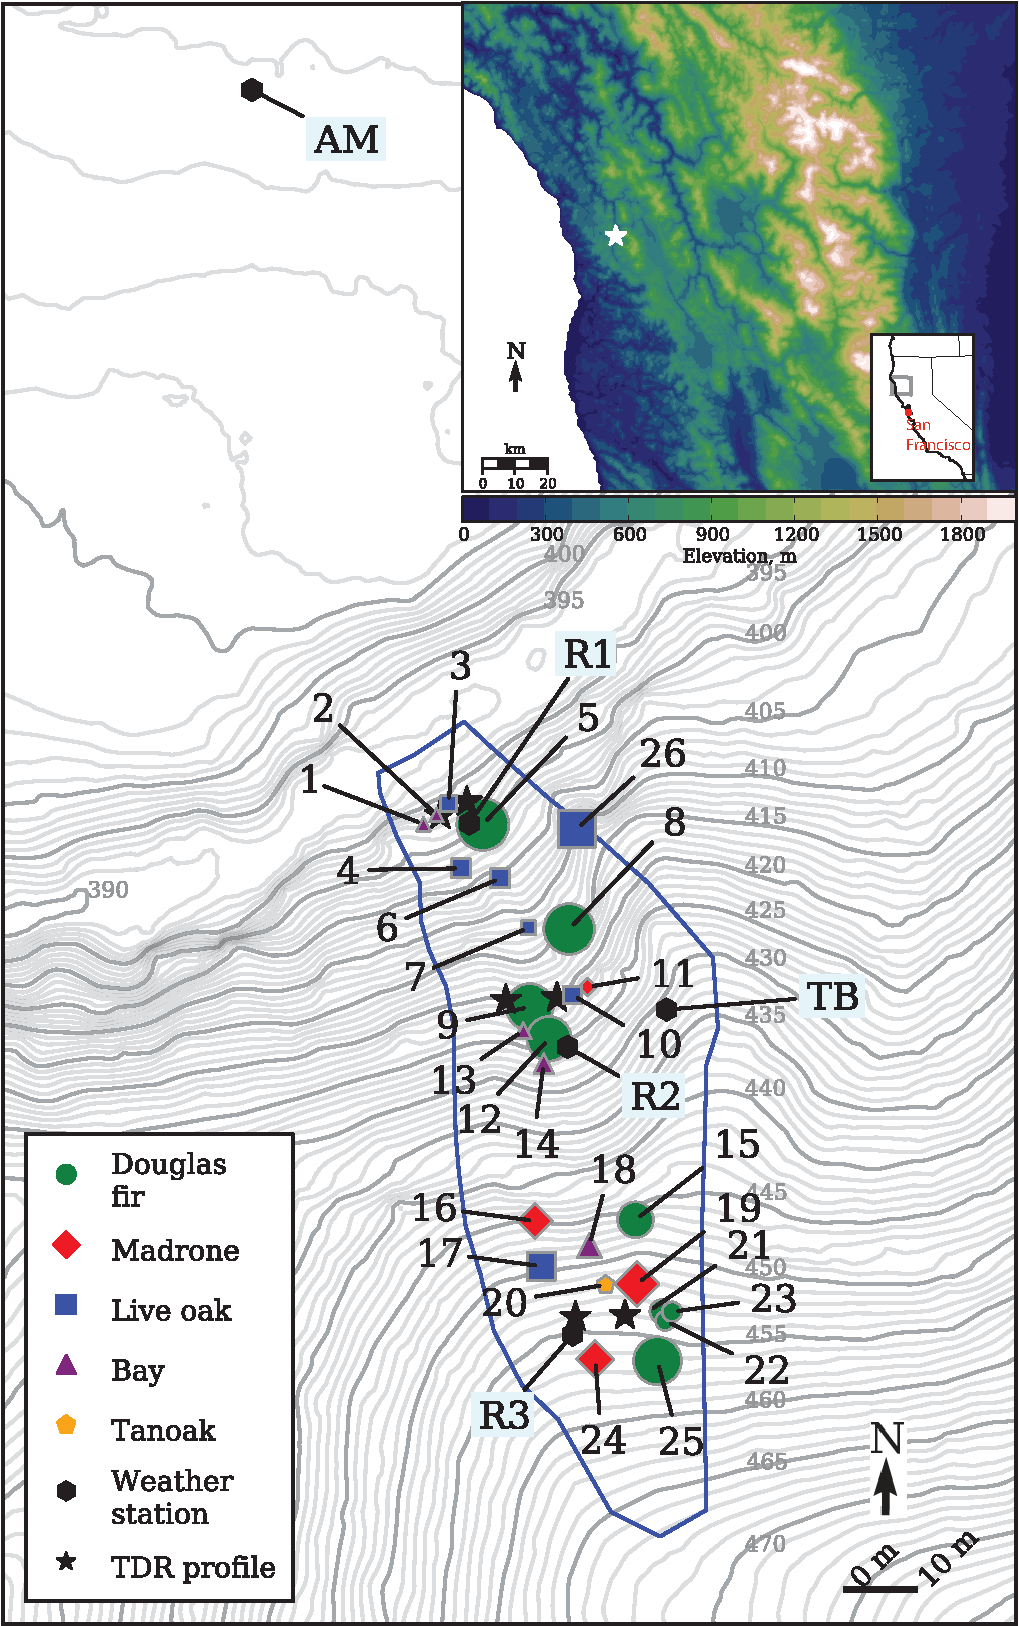
\includegraphics[width=0.7\textwidth]{ch1-sapflow/figures/Figure01.pdf}
\caption{Site map, showing topography, weather stations (R1, R2, R3, TB, AM), TDR profiles, and trees instrumented with sap flow sensors.  Symbols for instrumented trees are scaled by the tree diameter.  Tree numbers correspond with those in Table \ref{tbl:tree_props}.  Light gray numbers show elevation above sea level, in m.  Large inset: regional topography near the Angelo Coast Range Reserve (white star) [\cite{globe}].  Small inset: California, with gray box outlining the region displayed in the large inset, and red dot showing San Francisco.}
\label{fig:sapflow_map}
\end{figure}

The study site (39.729$^{\circ}$N, 123.644$^{\circ}$W) is located in the University of California Angelo Coast Range Reserve (ACRR) in Mendocino County, northern California, about 260 km north of San Francisco (Figure \ref{fig:sapflow_map} inset).  The ACRR sits in the Eel River watershed about 16 km east of the Pacific coast, just outside the coastal fog belt in the complex topography of the California Coast Range. The highest point in the ACRR, Cahto Peak, has an elevation of 1300 m above sea level, and the base elevation of the reserve is 400 m above sea level.
	
The field site, known as ``Rivendell'', is a small (4000 m$^2$), north-facing hillslope that drains to Elder Creek, a tributary of the South Fork Eel River (Figure \ref{fig:sapflow_map}).  Rivendell is the subject of an interdisciplinary collaborative project to study the lifecycle of water through a steep hillslope, and over 700 separate instruments have collected over 100 million data points between 2007 and May 2012.  The site has an average slope of approximately 32 degrees.  The subsurface structure consists of a thin soil mantle over a layer of highly fractured sedimentary rock, underlain by unweathered bedrock with very low permeability.  The fractured, weathered bedrock zone transitions with depth from relatively soil-like granular material to low-permeability bedrock bounded by fractures.  Both the soil mantle and the weathered rock layer are thicker at the hill crest (60 cm soil and 20 m weathered rock) and thinner at the base of the hill (0-30 cm soil and 5 m weathered rock) [\cite{rempe2010}].

The old-growth forest in the ACRR consists primarily of Douglas-fir (\textit{Pseudotsuga menziesii}), coast redwood (\textit{Sequoia sempervirens}), interior live oak (\textit{Quercus wislizeni}), tanoak (\textit{Notholithocarpus densiflorus}), Pacific madrone (\textit{Arbutus menziesii}), and California bay (\textit{Umbellularia californica}).  In the Eel River watershed, Douglas-fir constitutes approximately 40\% of tree basal area [\cite{woudenberg2010forest}] and is commonly associated with Pacific madrone, tanoak, live oak, and other species in the Pacific Douglas-fir alliance in coastal northern California [\cite{usda}].  At the study site, Douglas-firs form the overstorey, with heights up to 55-60 m, while live oaks, bays, Pacific madrones, and tanoaks form the lower canopy, reaching heights of approximately 20 m.  Below the lower canopy, there are smaller (5-10 m) trees of all species. There is no dense ground cover. Douglas-firs, live oaks, tanoaks, and bays are evenly distributed across the hillslope, while Pacific madrones occur more frequently upslope.  Douglas-fir is a needleleaf tree, while live oaks, tanoaks, Pacific madrones, and bays are broadleaf trees, but all of these species are evergreen. The rooting depths of trees at this site have not been determined, but during drilling of wells at the site, roots of unidentified species were observed most densely in the top several meters and with decreasing density to a depth of 15.2 m.

Climatic variables, including air temperature (\textit{T}, $^{\circ}$C), relative humidity (\textit{RH}, \%), solar radiation (\textit{I}, W/m$^2$), and precipitation (\textit{P}, mm), are measured at five weather stations at the site (Figure \ref{fig:sapflow_map}).  One weather station (TB) is located approximately 30 m above ground in the tree canopy, three weather stations (R1, R2, and R3) are located 1 m above the ground in an along-slope transect, and one weather station (AM) is located in an open meadow with full clearance, across the stream from the site.  The weather stations on the site (TB, R1, R2, and R3) are used here to characterize the \textit{VPD} at the site (\textit{T} and \textit{RH} from Vaisala HMP45C-L sensors at R1, R2, R3, and from a Vaisala WXT510 sensor at TB; Vaisala, Helsinki, Finland), while the meadow weather station (AM) is used for unobstructed \textit{I} and gross \textit{P} (Li-Cor LI200X-L pyranometer, Li-Cor, Lincoln, NE, USA; and Campbell Scientific TE525 tipping bucket rain gauge, Campbell Scientific, Logan, UT, USA).  All meteorological and soil moisture measurements were recorded with CR1000 dataloggers (Campbell Scientific) at intervals of 15 minutes until 2010 and 5 minutes beginning in 2010, and transmitted wirelessly and automatically to an online server; the entire system is powered only by solar cells.

Both shallow soil moisture and groundwater level are measured at Rivendell.  Depth profiles of $\theta$ (with a sensor placed every 5 to 10 cm down to a depth of 50 to 70 cm) are measured continuously with time domain reflectometer sensors (TDR; TDR100, Campbell Scientific) at six locations on the hillslope (Figure \ref{fig:sapflow_map}).  The TDR sensors are 7.5 cm long and are located in \textit{in situ} material: small trenches were dug in order to insert the probes horizontally into the soil or soil-like material in rock fractures, after which the trenches were backfilled with excavated material.  Measured dielectric values are converted to volumetric $\theta$ (m$^3$ water/m$^3$ total) using the standard Topp equation [\cite{topp1980electromagnetic}].  Groundwater level is monitored at 12 on-site wells.

Volumetric $\theta$ measurements are filtered to exclude values outside the sensor's valid range and averaged over each day to reduce noise (no diurnal cycle is evident at this site, in contrast to other Douglas-fir sites [\cite{brooks2006}; \cite{Warren:2007ly}]).  The daily-average values are then averaged across all depths for each profile; each profile average is normalized by its maximum to convert to relative $\theta$ (\%); and the six profiles on the slope are then averaged to produce a site-averaged $\theta$ time series.  The conversion to relative soil moisture is performed because no site-specific TDR calibration was performed.  We explain our reasoning for the site averaging in the Discussion, Section \ref{sec:sapflow_soilmoisture}.

\subsection{Sap flow measurement}
Sap velocity, the velocity of water through the xylem parallel to the axis of the tree trunk, is measured in 26 trees using 39 heat ratio method sensors (ICT International, Armidale, Australia; \cite{burgess2001improved}) installed 1 m above the ground in the tree trunks.  The tree locations, species, and diameters at breast height are shown in Figure \ref{fig:sapflow_map}, with the symbol size scaled by tree diameter, and the properties of each sensor are listed in Table \ref{tbl:tree_props}.  The trees were chosen to represent the distribution of tree species and sizes on the hillslope, within the constraints of accessibility on the steep slope and a limited number of sensors.  Multiple trees were instrumented for each species except tanoak (1 tree), which was sparse on this hillslope (uncharacteristically for this region.)  Before installing the sensors, bark was removed to the cambium from an approximately 5 cm x 5 cm area.  Each sensor measures the velocity of a heat pulse emitted by the sensor at two radial depths in the xylem: 12.5 mm and 27.5 mm.  These depths are not precise because of minor errors in sensor placement; errors in probe spacing are corrected using the procedure in \cite{burgess2001improved}.  For this procedure, we assume zero flow at times when water stress is expected to be minimal: pre-dawn (within 3 hours before sunrise), high relative humidity (between 92 and 95\%), no solar radiation, no daily rain, and between January and March.  Sensors were moved in late 2010 to minimize wounding, creating two stages of deployment (2009-2010, and 2011.)  Because we did not measure wound diameters around the probes (as that would be destructive), we assume a wound diameter of 0.2 mm (a central value from Table 1 in \cite{burgess2001improved}) for all sensors; the wound correction is a linear factor and is thus removed by the normalization described below (Section \ref{sec:normalization}).  Heat pulse velocity was recorded on ICT SL5 Smart Loggers (ICT International, Armidale, Australia) at 30-minute intervals.

\begin{table}
  \caption{Sap flow sensor properties, including tree, sensor ID, stage of deployment, species, DBH (diameter at breast height), nearest weather station, active depth (radial sensor position with larger sap velocity), 99.5th percentile instantaneous sap velocity for each sensor position, 12.5 mm - 27.5 mm sensor correlation ($R^2$ coefficient comparing velocities at the two measured radial positions), 99.5th percentile daily integral sap velocity for the active sensor depth, lag time of sap velocity relative to radiation, lag time of sap velocity relative to $VPD$, wood dry density at the two sensor positions, and wood water content at the two sensor positions.}
  \label{tbl:tree_props}
  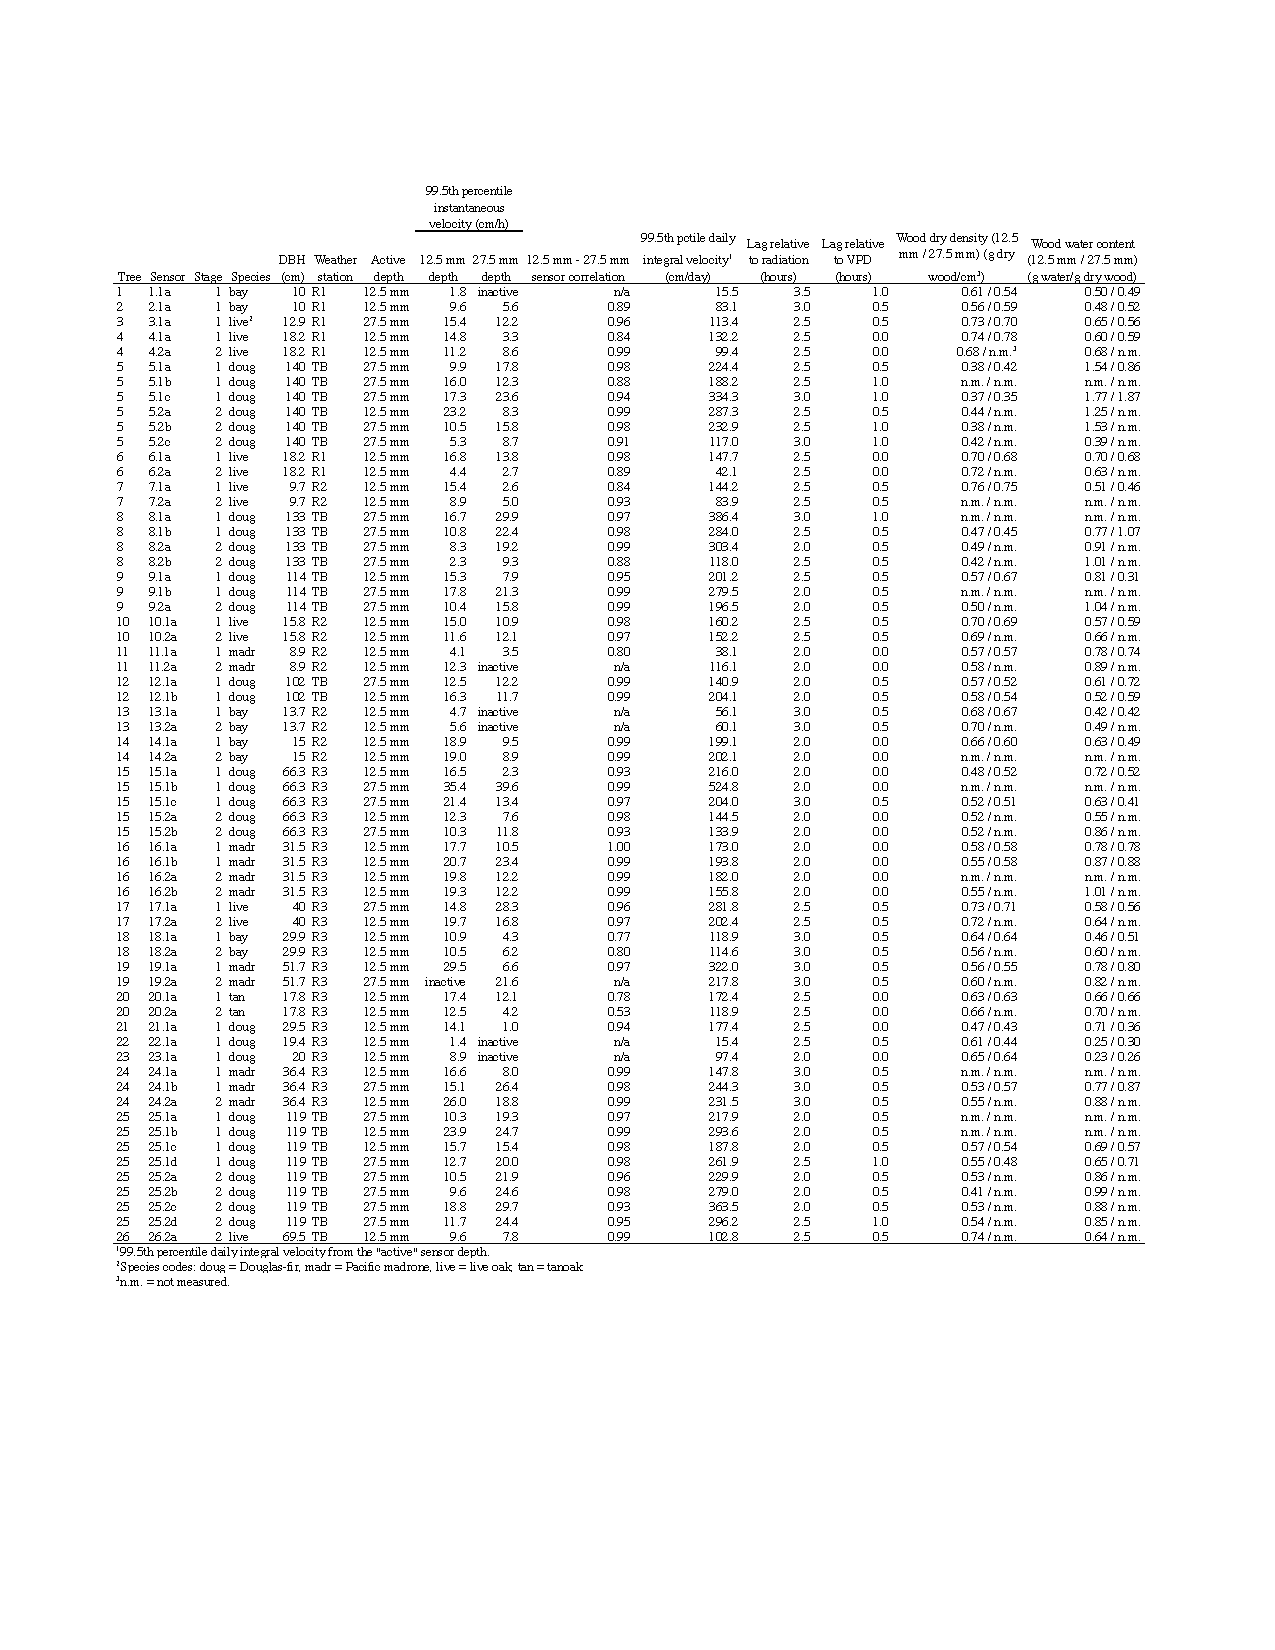
\includegraphics[width=\linewidth]{ch1-sapflow/tables/Table1_cropped.pdf}
\end{table}

Wood density and water content were measured by taking cores with an increment borer in October 2010 and October 2012, and these properties are used to convert heat pulse velocity to sap velocity [\cite{burgess2001improved}].  For several sensors, wood density and water content were not measured (Table \ref{tbl:tree_props}); for these sensors, the species-averaged values were used.  Because water content was only measured once at the end of each stage, we used a constant value throughout the year.  Uncertainties associated with this assumption are discussed in Section \ref{sec:sapflow_soilmoisture}.

For the following analyses, for each sensor, the depth with the larger magnitude of velocity (i.e. the most ``active'' depth) is chosen.  Sap velocity is known to vary radially through the sapwood [\cite{cohen1985determination}; \cite{vcermak1992radial}; \cite{nadezhdina2002radial}; \cite{ford2004assessing}]; in our measurements, the velocities at 12.5 mm and 27.5 mm differed in magnitude but were highly correlated for almost all sensors ($R^2$ values listed in Table \ref{tbl:tree_props}); as such, we include only one depth per sensor in order to avoid redundancy.

Finally, we add the caveat that we treat sap velocity as proportional to transpiration.  We discuss this assumption in Section \ref{sec:sapflow_soilmoisture}.

\subsection{Normalization}
\label{sec:normalization}
For most of our analyses, we use normalized sap velocities.  Normalizing allows us to compare temporal dynamics and environmental responses between sensors with very different absolute magnitudes, and eliminates the time-invariant differences in absolute velocity due to azimuthal, radial, or between-tree variation in wood properties.  We employ normalization on two time scales.   The first normalizes instantaneous (30-minute frequency) measurements by dividing by the 99.5th percentile value of that sensor (to avoid normalizing by an outlier); this normalization is used for analyzing responses to environmental drivers (Sections \ref{sec:mcmc} and \ref{sec:envresponse}).  In the second, daily integrals of sap velocity are normalized by dividing by the 99.5th percentile daily integral for each sensor; the normalized daily integrals are used for analyzing seasonal dynamics (Sections \ref{sec:pca} and \ref{sec:seasonal}), since the diurnal cycle is removed.  Sensors are normalized separately for each stage of deployment, because azimuthal variations in wood properties caused differences in absolute magnitude of velocity when sensors were moved within a tree.

\subsection{Principal Component Analysis}
\label{sec:pca}
We use principal component analysis (PCA) to find the dominant spatial and, importantly, temporal sap flow patterns in the sap flow dataset, and to compare the dominant seasonality patterns between trees, across space and between species.  PCA, also known as empirical orthogonal function analysis [\cite{lorenz1956empirical}], reduces a dataset with many points in space and time to a few orthogonal patterns that explain most of the variance. These orthogonal patterns are determined empirically from the data, as the eigenvectors of the covariance matrix.  PCA yields a series of temporal functions (PCs), with a corresponding series station weighting factors (EOFs), which represent how strongly each time function (PC) contributes to the actual time series at a given station.  The pairs of time-space functions (PC$_m$ and EOF$_m$) are ordered by the fraction of the total dataset variance that each explains.

We perform PCA separately on each of the two stages of sensor deployment (2009-2010, and 2011), because many of the time series were discontinuous across the sensor move; many sensors failed after the move or were placed in roots, which were not analyzed in the present study.  In order to maximize the amount of data included in the analysis, we performed PCA on the two stages separately.  Performing PCA on the two stages also has the advantage of providing replication of the dominant patterns of variability; similarity between results from the two stages would indicate interannual robustness of the seasonal patterns.

Days with missing data are excluded.  The analyses are performed on normalized daily integral values, subtracting each sensor's mean for the analysis period to focus on the temporal variability. The analysis is performed in Python, using the NumPy linalg function \textit{eig}. In the following, we focus on the first two PC-EOF pairs for each analysis, as they together explain over 90\% of the variance.

\subsection{MCMC estimation of environmental response parameters}
\label{sec:mcmc}
We quantify the relationship between each sensor's instantaneous sap flow and environmental drivers using the Jarvis model [\cite{jarvis1976interpretation}], which parameterizes stomatal conductance in terms of empirical functions of \textit{VPD}, \textit{I}, and $\theta$.

We begin with the assumption that each sensor's instantaneous normalized sap velocity ($v_n$, unitless) is proportional to the tree's transpiration ($E$, liters/day), scaled by a multiplier, $\alpha$ (liters/day), the product of maximum sap velocity, sap wood cross-sectional area, and the profile of sap velocity as a function of radius:

\begin{equation} % equation 1
\label{eqn:sf1}
E = \alpha \cdot v_n.
\end{equation}

Transpiration also equals the product of the tree's bulk canopy conductance ($g_c$, liters/day/kPa) and the leaf-to-air vapor pressure difference (which we approximate with the air \textit{VPD}.)  Thus,

\begin{equation} % equation 2
E = g_c \cdot VPD.
\end{equation}

Following the Jarvis model, canopy conductance ($g_c$) is modeled as a maximum conductance ($g_{cmax}$, liters/day/kPa), reduced by empirical multiplicative functions, ranging from 0 to 1, of important environmental modifiers: \textit{VPD}, $\theta$, and $I$ [\cite{jarvis1976interpretation}; \cite{oren1999survey}; \cite{waring2011generalizing}].

\begin{equation}  % equation 3
\label{eqn:sapflow_jarvis_simple}
g_c = g_{cmax} \cdot f_{VPD}(VPD) \cdot f_{\theta}(\theta) \cdot f_I(I).
\end{equation}

The functions of environmental modifiers are analytical parameterizations based on previous empirical observations.  For the atmospheric evaporative demand function, $f(VPD)$, we use an asymptotic function [\cite{lohammar1980fast}; \cite{lindroth1986numerical}; \cite{dang1997regulation}],

\begin{equation}  % equation 4
\label{eqn:sapflow_fVPD}
f_{VPD}(VPD) = \frac{1}{1+VPD/D_o},
\end{equation}
where $D_o$ (kPa) describes the sensitivity of $g_c$ to \textit{VPD}.

The water supply function, $f(\theta)$, is modeled as a sigmoid function, chosen because it is a continuous function that represents the threshold limitation of transpiration by $\theta$ in very dry soils; this is a continuous functional form that approximates the piecewise-linear Feddes model [\cite{feddes}; \cite{chen2008observations}]:

\begin{equation}  % equation 5
\label{eqn:sapflow_soilmois}
f_{\theta}(\theta) = \frac{1}{1+\exp(-\beta(\theta-\theta_o))},
\end{equation}
where $\beta$ (unitless) measures the rate of decrease of transpiration at low $\theta$, and $\theta_o$ (unitless) is the value of $\theta$ at which the transpiration decline is centered.  These parameters can be related to the more standard stress point and wilting point of the Feddes model by estimating the $\theta$ at which the sigmoid function begins to decline (the stress point) and the $\theta$ at which the sigmoid function is approximately zero (the wilting point.)

The radiation function, $f(I)$, is modeled as a linear function, after \cite{waring2011generalizing}:

\begin{equation}  % equation 6
f_I(I) = \gamma \cdot (I-1000 \, {\rm W/m^2})+1,
\end{equation}
where $\gamma$ ((W/m$^2$)$^{-1}$) is the sensitivity of transpiration to \textit{I}, and $f(I)$ is prescribed to be maximum (equal to 1) at maximum \textit{I} (1000 W/m$^2$).

Thus, we model normalized sap velocity as a function of \textit{VPD}, $\theta$, \textit{I}, and five parameters (considering $g_{cmax}/\alpha$ (kPa$^{-1}$) as a single parameter):

% equation 7
\begin{align}
\label{eqn:sapflow_jarvis}
v_n & =  \frac{g_{cmax}}{\alpha} \cdot VPD \cdot f_{VPD}(VPD) \cdot f_{\theta}(\theta) \cdot f_I(I) \nonumber \\ 
& =  \frac{g_{cmax}}{\alpha} \cdot \frac{VPD}{1+\frac{VPD}{D_o}} \cdot \frac{1}{1+\exp(-\beta(\theta-\theta_o))} \cdot (\gamma \cdot (I-1000)+1).
\end{align}

We estimate these five parameters for each sensor using a Markov chain Monte Carlo (MCMC) method, described in the appendix (Section \ref{sec:sapflow_appendix}).  The MCMC method allows us to quantify uncertainty in the parameters and avoid local minima traps on the complex $\chi ^2$ surface that might hinder optimization algorithms.  Each sap flow sensor is matched with the nearest weather station: the canopy weather station (TB) is used for the overstorey trees, while the nearest ground station (R1, R2, or R3) is used for the understorey canopy trees, including small Douglas-firs.  Incoming \textit{I} measured in the open meadow (station AM, Figure \ref{fig:sapflow_map}) is used for all sensors, because \textit{I} was only measured at station AM.  \textit{VPD}, \textit{I}, and $\theta$ were subsampled to the 30-minute frequency of sap flow measurements.  For each tree, sap velocity is lagged relative to \textit{I} and \textit{VPD} by a lag time determined by the maximum lag correlation for that tree's average timeseries, similar to the procedure in \cite{dragoni2009decoupling}; lag times are listed in Table \ref{tbl:tree_props}.  The analysis is performed using times when \textit{I} was greater than zero (i.e., daytime observations) and \textit{VPD} was greater than 0.1 kPa.  Days with more than 2 mm of rain were excluded, because on those days leaves were probably covered with water and sap velocity thus was probably not controlled by stomatal response to the environment.  The site-averaged, daily-averaged $\theta$ is used for all sensors, as described in Section \ref{sec:sapflow_sitedesc}.  Parameters are also estimated for each species as a whole, using the average $v_n$ at each measurement from all sensors from a given species; these are referred to as the ``species-averaged timeseries" parameters.

\subsection{Estimates of regional transpiration}
\label{sec:sapflow_regmeth}
We use the species-averaged timeseries of normalized sap velocity, along with Forest Inventory and Analysis (FIA) [\cite{woudenberg2010forest}] observations of tree size and species distributions in the Eel River watershed, to estimate the contribution of each species to regional transpiration.  We estimate regional transpiration, rather than hillslope transpiration at our particular site, because regional distributions of trees by species and diameter are available from the FIA inventory, but no species-diameter inventory has been conducted at our particular site.  This scale jump requires simplifications and assumptions (described below), and as such, our calculations are a rough best estimate and an attempt to bound the range of possible forest transpiration in this region from a bottom-up perspective.  

Transpiration was estimated using Equation \ref{eqn:sf1}, with $v_n$ calculated using the species-averaged timeseries Jarvis parameters, and $\alpha$ disaggregated as follows.  Transpiration for a single tree ($E_{tree}$, cm m$^2$/hr) is

% equation 8
\begin{align}
E_{tree} & = \int_{r_{inner}}^{r_{outer}} 2\pi r \, v(r) \, \mathrm{d}r \nonumber \\ 
& =  \int_{r_{inner}}^{r_{outer}}  2\pi r \, v_{max} \, v_{n} \, f_{prof}(r) \, \mathrm{d}r,
\end{align}
where $r$ is radial position on a cross-section of the tree, $r_{inner}$ is the radial position of the sapwood-heartwood boundary (meters), $r_{outer}$ is the radial position of the sapwood-bark boundary (meters, here treated as approximately equal to half the tree diameter at breast height, $d/2$), $v(r)$ is the sap velocity as a function of radial position in the sapwood (cm/hr), and $f_{prof}(r)$ is a linear function between 0 and 1 describing the radial profile of sap velocity relative to the velocity at the outer edge (described below).  In this equation, $v_n$ and $v_{max}$ can be pulled out of the integral, and the resulting term $2\pi \, v_{max} \, \int_{r_{inner}}^{r_{outer}}  r \, f_{prof}(r) \, \mathrm{d}r$ is equal to $\alpha$ in Equation \ref{eqn:sf1}.

The thickness of the sapwood is estimated using two site-specific sapwood thickness--diameter relations, derived from 21 tree cores taken near Rivendell (15 Douglas-fir samples ($R^2=0.88$) and 6 Pacific madrone samples ($R^2=0.83$)):
\begin{align}
\label{eqn:sapwood}
w_{sap,Douglas-fir} = 0.12d+0.0089\\
w_{sap,madrone} = 0.1d+0.0071 ,
\end{align}
and
\begin{equation}
r_{inner} = d/2-w_{sap},
\end{equation}
where $w_{sap}$ is sapwood thickness (m).  Our Douglas-fir relationship is roughly similar to the one found by \cite{smith1966variation} for Douglas-fir.  

In addition, for other broadleaf species, we use the ring-porous equation from \cite{wullschleger2001transpiration}:
\begin{equation}
\label{eqn:sapwood2}
r_{inner,Wullschleger} = \sqrt{\left(\frac{d}{2}\right)^2-\frac{1.637d^{0.56}}{\pi}}.
\end{equation}
This equation is used for non-Pacific-madrone broadleaf species.

Sap velocity was approximated as a linear function of radial position in the sapwood, based on observations that sap velocity is often lower in the inner sapwood than in the outer sapwood [\cite{ford2004assessing}; \cite{cohen1985determination}; \cite{vcermak1992radial}; \cite{nadezhdina2002radial}].  The velocity at the outer edge of the sapwood was estimated as the product of a time-invariant maximum velocity ($v_{max}$, cm/hr) and a time-varying normalized velocity ($v_n$, unitless), approximated as the species-averaged timeseries of measured normalized sap velocity.  $v_{max}$ values for each species were treated as independent of tree diameter and were approximated with the species-averaged maximum instantaneous velocities from Table \ref{tbl:sapflow_maxvel}.  Sap velocity is assumed to be independent of azimuth, or equivalently, we assume that $v_{max,sp}$ is an average of the maximum velocity around the bole of a tree.

\begin{table}
  \caption{Species-averaged maximum sap velocities.}
  \label{tbl:sapflow_maxvel}
  \begin{tabular}{l r}
  \hline
  Species & Velocity (cm/h) \\
  \hline
  Douglas-fir & 18.2 \\
  Pacific madrone & 19.5 \\
  live oak & 14.0 \\
  bay & 10.1 \\
  tanoak & 15.0 \\
  \hline
  \end{tabular}
\end{table}

Because the radial profile of sap velocity is not well constrained with our measurements, we test three possible velocity profiles, with $v(r) = v_{max} \, v_n \, f_{prof}(r)$: (1) constant velocity across the sapwood ($f_{prof}(r) = 1$); (2) velocity decreasing linearly from $v_{max} \, v_n$ at the outer edge of the sapwood to $0.5 \, v_{max} \, v_n$ at the inner edge of the sapwood ($f_{prof}(r) = 1+\tfrac{0.5}{w_{sap}}(r-r_{outer})$ ); and (3) velocity decreasing linearly from $v_{max} \, v_n$ at the outer edge of the sapwood to 0 at the inner edge of the sapwood ($f_{prof}(r) = 1+\tfrac{1}{w_{sap}}(r-r_{outer})$ ).

Transpiration is scaled from a single tree to the regional scale using distributions of tree species and sizes measured in the Eel River watershed by the FIA program, binned by diameter in 5 cm bins [\cite{woudenberg2010forest}] (locations of FIA plots are intentionally ``fuzzed and swapped'' for privacy reasons, but the provided coordinates are ``similar'' to the true coordinates with an unspecified offset).  The FIA surveyed 321 forested plots within the Eel Watershed.  Figure \ref{fig:sapflow_abundances} shows $N_{i,sp}$, the number of trees per km$^2$ in each diameter bin ($i$) for major species categories in the watershed ($sp$), averaged over the 321 FIA plots.

\begin{figure}[here]
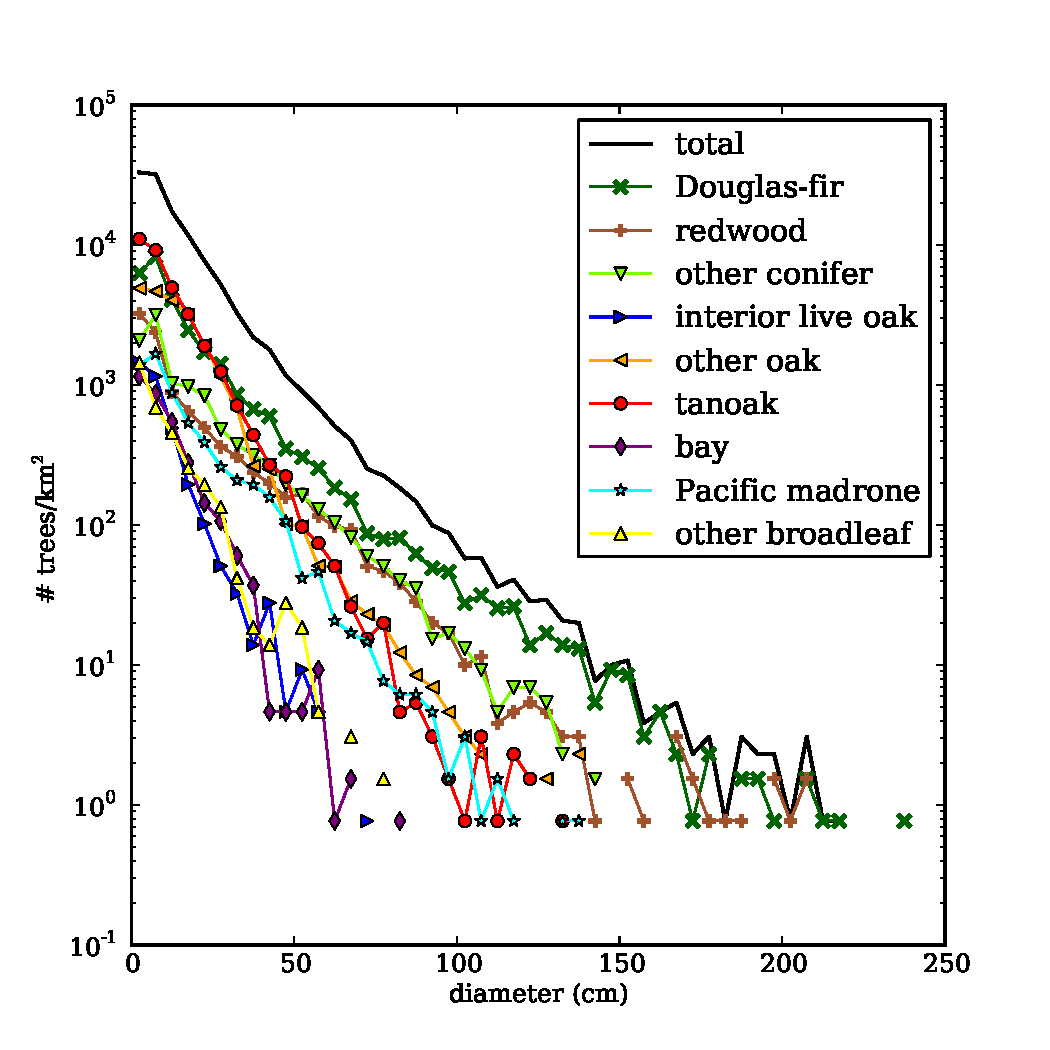
\includegraphics[width=0.9\textwidth]{ch1-sapflow/figures/Figure02.pdf}
\caption{Counts of trees per km$^2$ in major species categories, binned diameter; from FIA plots in the Eel River watershed [\cite{woudenberg2010forest}].  The category ``other conifer'' includes knobcone pine, Jeffrey pine, sugar pine, Western white pine, bishop pine, ponderosa pine, California foothill pine, white fir, grand fir, red fir, Pacific yew, western hemlock, incense cedar, and Sitka spruce.  The category ``other oak'' includes California live oak, canyon live oak, blue oak, Oregon white oak, California black oak, and California white oak.  The category ``other broadleaf'' includes bigleaf maple, California buckeye, red alder, white alder, giant chinkapin, and bitter cherry.}
\label{fig:sapflow_abundances}
\end{figure}

Regional transpiration due to each species (mm/d) is then estimated by summing individual tree transpiration of the species over all diameter bins ($i$):
\begin{align}
\label{eqn:transpreg}
T_{sp} &= \sum_{i} N_{i,sp} \, E_{tree,i,sp} \nonumber \\
&= 2\pi \, v_{max,sp} \, v_{n,sp} \, \sum_{i} N_{i,sp} \, \int_{r_{inner,i}}^{r_{outer,i}}  r \, f(r) \, \mathrm{d}r ,
\end{align}
and subsequently applying a unit conversion factor of $(10 \tfrac{mm}{cm}) (24 \tfrac{hr}{day}) (10^{-6} \tfrac{km^2}{m^2})$.  Total regional transpiration is estimated by summing transpiration estimated for all species, using the averaged time series of measured species to represent unmeasured but similar species.  All conifers, including redwoods, are assigned the Douglas-fir time series; all oaks, both evergreen and deciduous, are assigned the interior live oak time series; and all other unmeasured broadleaf trees are assigned the Pacific madrone time series, in order to give an upper-bound estimate on dry season transpiration.  Thus, we effectively bin species into categories of needleleaf evergreen and broadleaf evergreen; these assumptions are necessary because redwoods and major pine species were not measured due to their scarcity at our site.  In addition, we calculate regional transpiration in two extreme hypothetical cases, using the FIA total tree size distribution (black line in Figure \ref{fig:sapflow_abundances}): one case in which all trees are assigned the Douglas-fir time series, and another case in which all trees are assigned the Pacific madrone time series. 

The sap-flow-based regional transpiration estimates are compared with remotely-sensed MODIS-derived estimates of ET [\cite{mu2007development}].  The MODIS algorithm uses remotely-sensed LAI and modeled stomatal response based on an assigned plant functional type (which for this region is evergreen needleleaf forest), combined with meteorology from atmospheric reanalysis, to estimate stomatal conductance and ET.  No soil moisture or subsurface information is explicitly included.  Two spatial scales of the MODIS-derived estimate are presented: the 1 km x 1 km pixel nearest to Rivendell (pixel centered about 450 m east of Rivendell), and the average for all pixels in the Eel River watershed.  Our goals in comparing our estimated to the MODIS-derived estimate are a) to confirm that our estimates are the right order of magnitude, and b) to compare the seasonal timing of transpiration between the methods.



\section{Results}

\subsection{Environmental conditions}

\begin{figure}[here]
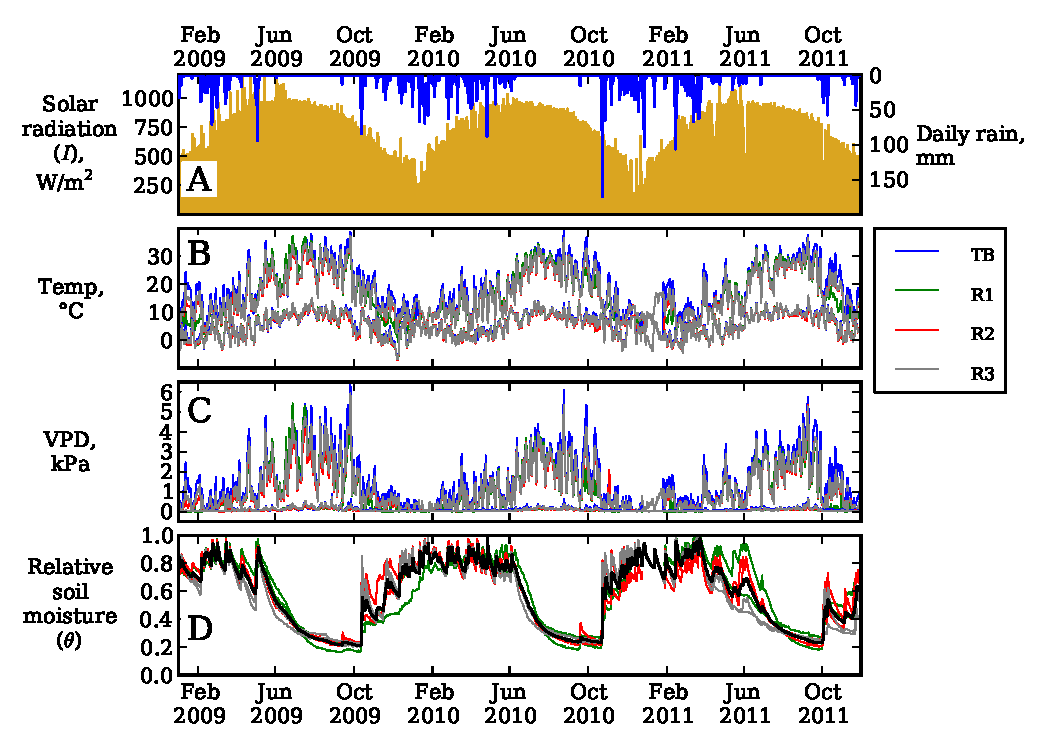
\includegraphics[width=0.9\textwidth]{ch1-sapflow/figures/Figure03.pdf}
\caption{Climatic and hydrologic time series: (a) solar radiation (\textit{I}, yellow) and daily rainfall (blue), both measured unobstructed in an open field; (b) daily minimum and maximum air temperature (\textit{T}) at ground stations (R1, R2, R3) and canopy station (TB); (c) daily minimum and maximum vapor pressure deficit (\textit{VPD}) at ground stations (R1, R2, R3) and canopy station (TB); (d) red, green, and gray: daily average relative soil moisture (\textit{$\theta$}), averaged over each of the 6 profiles shown in Figure \ref{fig:sapflow_map} (colors indicate the profile's nearest weather station, as in panel (b) legend); black: average of the 6 profile averages of relative soil moisture.}
\label{fig:sapflow_met}
\end{figure}

The ACRR has a Mediterranean climate with a marked winter wet season and summer dry season.  The wet season at the ACRR extends from approximately October through April (90\% of the annual precipitation fell in these months in 2009-2011), and very little rain falls during July through September (less than 1\% in 2009-2011; Figure \ref{fig:sapflow_met}(a)).  Clear sky \textit{I} is maximum in late June (summer solstice) and minimum in late December (winter solstice), and \textit{I} can be reduced by 50 to 90\% on cloudy days.  The annual cycle of \textit{T} lags behind that of \textit{I}, with a peak in July and August and a minimum in January or February. The mean July-September \textit{T} for 2009-2011 was 18$^{\circ}$C, and the mean December-February \textit{T} was 5$^{\circ}$C (weather station R3).  The annual cycle of \textit{VPD} follows that of \textit{T} and also peaks in July or August.  \textit{T} and \textit{RH} vary somewhat along the hillslope: on clear days, the air is warmer and drier in the upper canopy and upslope, and the air is cooler and more humid downslope (up to 10$^{\circ}$C cooler at downslope ground level than in the canopy at midday in winter; Figure \ref{fig:sapflow_met}(b) and (c)).  Mean annual \textit{P} in the vicinity of the ACRR (National Climatic Data Center GHCN precipitation station USC00048490, 18 km NNE of the ACRR; data from 1960-2000; XXXX \textit{Williams et al.} [2012]) is 1800 mm, with significant interannual variability (standard deviation of 500 mm); on average, 3\% ($\pm$3\% standard deviation) of annual precipitation falls in July through September.  During the study period, precipitation at Rivendell ranged between a minimum of 1500 mm in water year 2008-2009 and a maximum of 2100 mm in water year 2010-2011.

Water storage below ground is also highly seasonal. The water table, measured by 12 on-site wells, remains near 5 m below ground throughout the year at downslope wells, but upslope it ranges from $\sim$10 m below ground in the wet season to $\sim$20 m below ground in the dry season.   Soil moisture ($\theta$) is high and dynamic during the winter rainy season but dries to fairly steady and very low values during the summer dry season (Figure \ref{fig:sapflow_met}(d); \cite{salve2012rain}).  

\subsection{Sap velocities}

\begin{figure}[here]
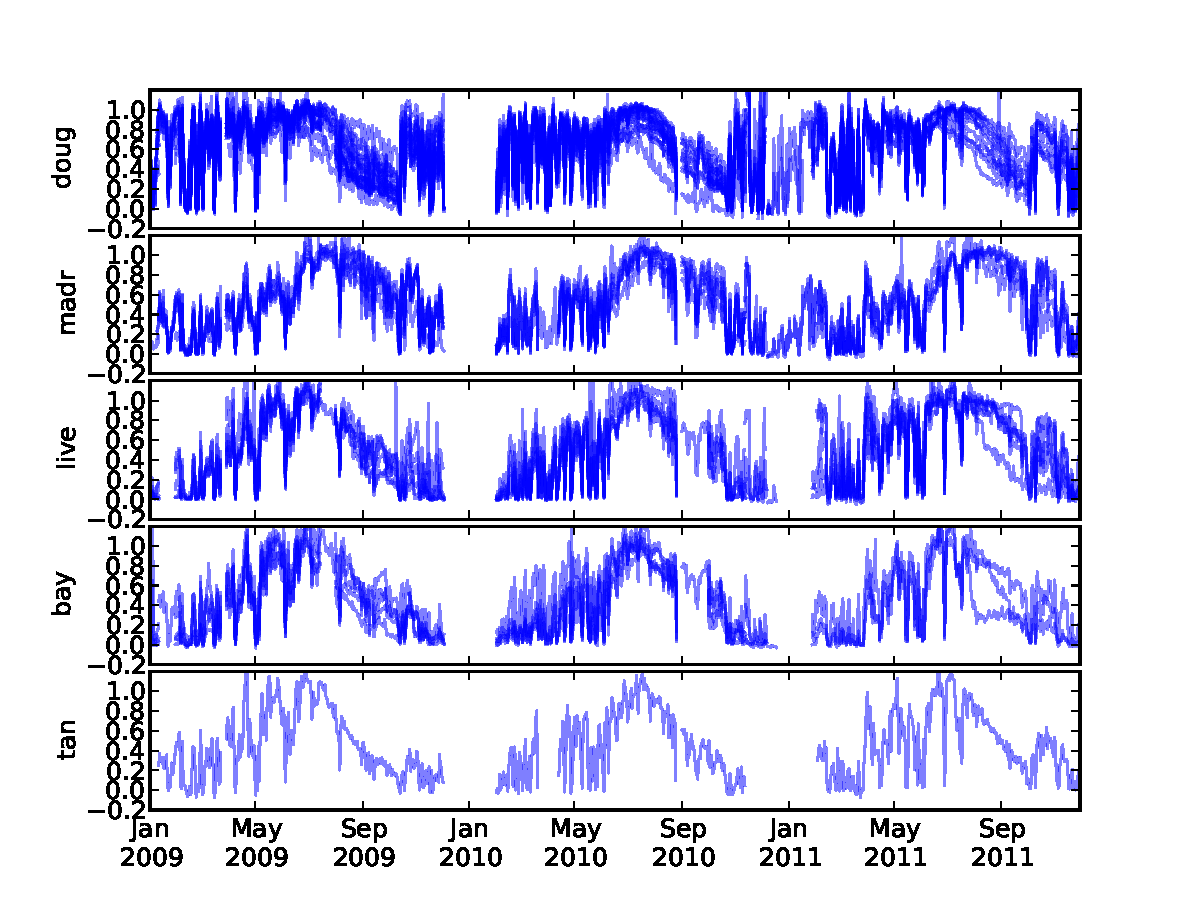
\includegraphics[width=0.9\textwidth]{ch1-sapflow/figures/Figure04.pdf}
\caption{Daily maximum normalized sap velocities for each sensor, separated by species.  Each sensor's line is slightly transparent, so that overlapping lines create darker blue colors.  Data gaps are due largely to power failure during times of low insolation.  Species codes: doug=Douglas-fir; madr=Pacific madrone; live=interior live oak; tan=tanoak.}
\label{fig:sapflow_normvel}
\end{figure}

The 99.5th percentile velocities for each sensor and each stage are listed in Table \ref{tbl:tree_props}, and the timeseries of daily maximum normalized instantaneous velocity for each sensor are shown in Figure \ref{fig:sapflow_normvel}, separated by species (only the daily maximum is shown for visibility.)  For the following analyses, we constructed tree-averaged timeseries for trees with multiple sensors by averaging the normalized velocities at each measurement time for all sensors in a given tree.  This tree-averaging was performed because sensors within a tree covaried strongly for all trees (Table \ref{tbl:sapflow_covar}), and thus sensors in the same tree were not independent.

\begin{table}
  \caption{Covariation of sap velocities within the same tree.}
  \label{tbl:sapflow_covar}
  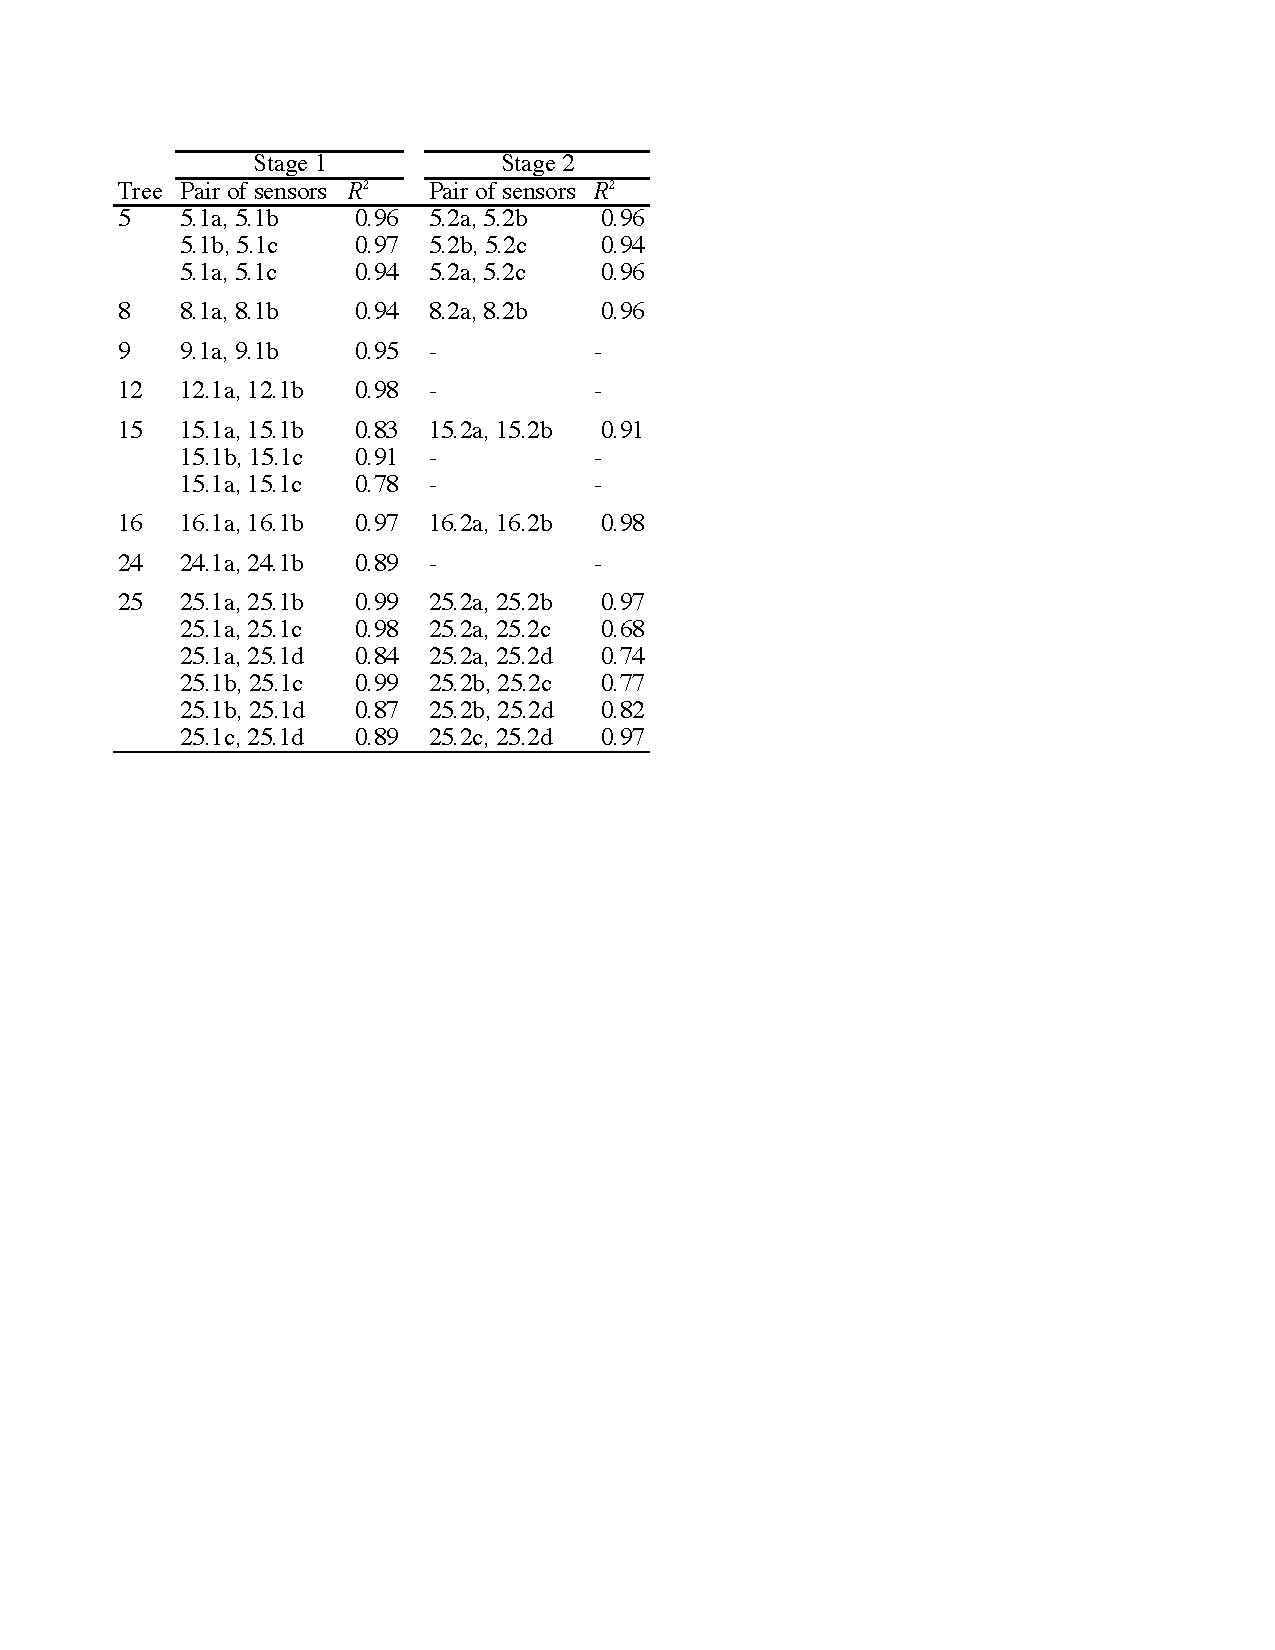
\includegraphics[width=\linewidth]{ch1-sapflow/tables/TableA1.pdf}
\end{table}

\subsection{Seasonal patterns: Principal Component Analysis}
\label{sec:seasonal}

\begin{figure}[here]
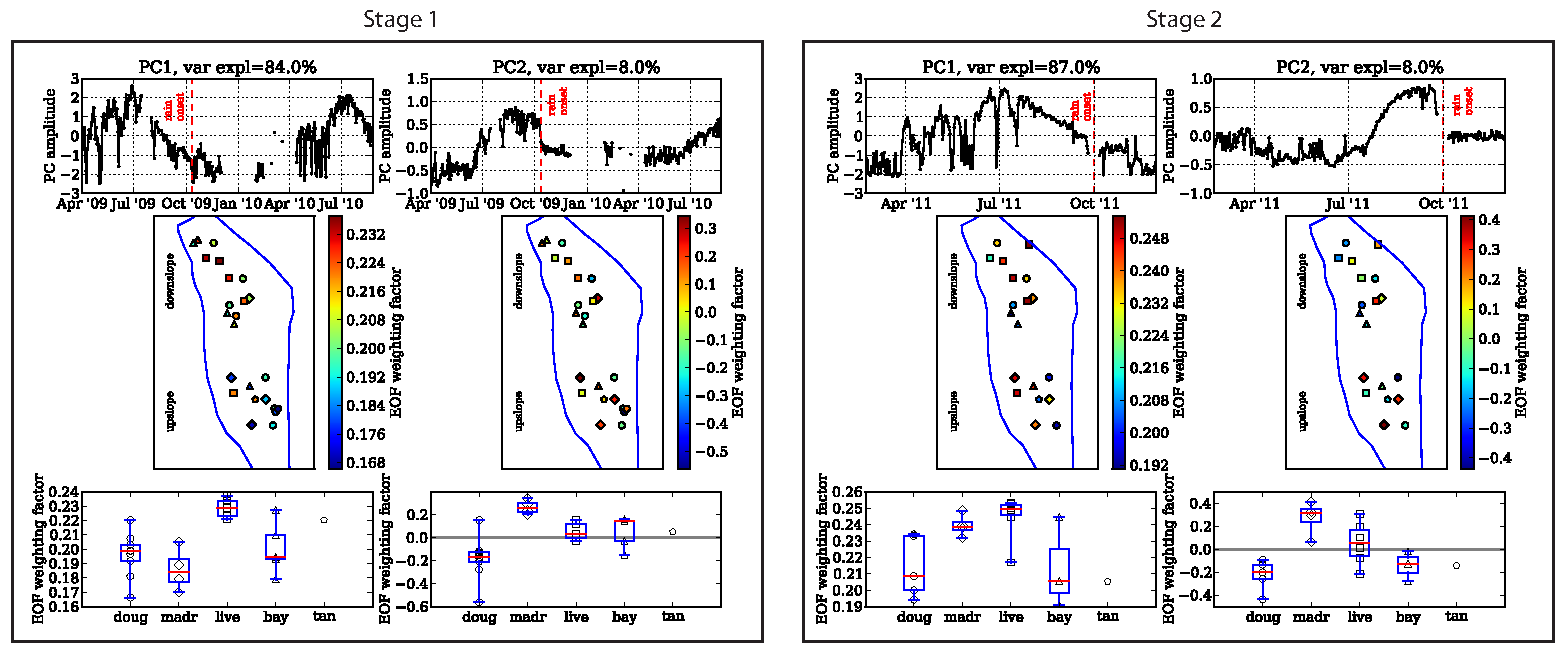
\includegraphics[width=0.9\textwidth]{ch1-sapflow/figures/Figure05.pdf}
\caption{PCA results for all sensors, for stage 1 (left box) and stage 2 (right box).  Within each stage, left column: PC/EOF 1, right column: PC/EOF 2.  Top row: principal component time patterns.  Circles show days included in the analysis.  Gaps represent periods of missing data longer than 4 days.  Middle row: maps of EOF weighting factors for all trees included in the analysis.  Symbol shape indicates species, as in Figure \ref{fig:sapflow_map}.  Bottom row: EOF weighting factors, sorted by species.  Box plot divides the quartiles of the distribution; red line shows the median.  Both the PCs and EOFs are unitless, because the analysis used normalized velocities.}
\label{fig:sapflow_eof}
\end{figure}

The time pattern that explains the most variance among all sap flow sensors, PC1, represents the common annual cycle, with a peak in early July and lower values through the winter, mirroring the annual cycle of solar radiation (Figure \ref{fig:sapflow_eof}, left column in each stage).  PC1 also contains the abrupt drops in sap flow on rainy days in winter and spring, when almost all sensors have very low sap velocity.  The annual cycle pattern is evident in PC1 for both stages, and PC1 explains 84\% of the variance in stage 1 (2009-2010) and 87\% of the variance in stage 2 (2011).  All sensors in both stages have positive weighting factors for PC1, meaning that all sensors display a component of this annual cycle pattern.  In stage 1, downslope trees tend to resemble PC1 more strongly than do upslope trees (i.e., have larger positive weighting factors).

The time pattern that explains the next-largest fraction of the variance, PC2, acts as a phase offset from the PC1 annual cycle, with a positive peak in the July-October dry season and negative values for the rest of the year (Figure \ref{fig:sapflow_eof}, right column in each stage).  Again, the PC2 pattern is similar between the two stages of deployment.  A positive EOF2 weighting factor for PC2 indicates greater July-October transpiration than PC1 and less November-June transpiration, and thus a shift in the peak season of transpiration later into the dry season.  On the other hand, a negative EOF2 weighting factor indicates less July-October transpiration compared to PC1 and greater transpiration in the rest of the year, and thus indicates a shift in peak transpiration earlier toward the wet spring.  PC2 explains 8\% of the variance in both stages.

The direction of the transpiration phase shift is species-specific.  Pacific madrones have the most positive weighting factors for PC2 in both stages, indicating a phase shift of peak transpiration later into the dry season (Figure \ref{fig:sapflow_eof}, bottom right panel in each stage).  Douglas-firs, in contrast, almost all have negative values, indicating a phase shift earlier toward the wet spring season.  Live oaks, bays, and the tanoak have weighting factors closer to zero, indicating less phase shift away from the PC1 pattern.

Additionally, the PC2 time pattern shows an abrupt decrease at the onset of the rainy season in October of each year.  Thus, Pacific madrone sap velocities, with positive PC2 amplitudes, decrease sharply at the onset of the rainy season, while Douglas-fir velocities, with negative PC2 amplitudes, increase sharply.

\subsection{Sensitivities to environmental drivers}
\label{sec:envresponse}

These PC/EOF patterns are empirical, indicating the dominant patterns of variability and demonstrating that there is a seasonal offset of transpiration between evergreen tree species at this site.  In order to investigate the drivers of this difference, we quantify the response of sap velocity to environmental variables.

\begin{figure}[here]
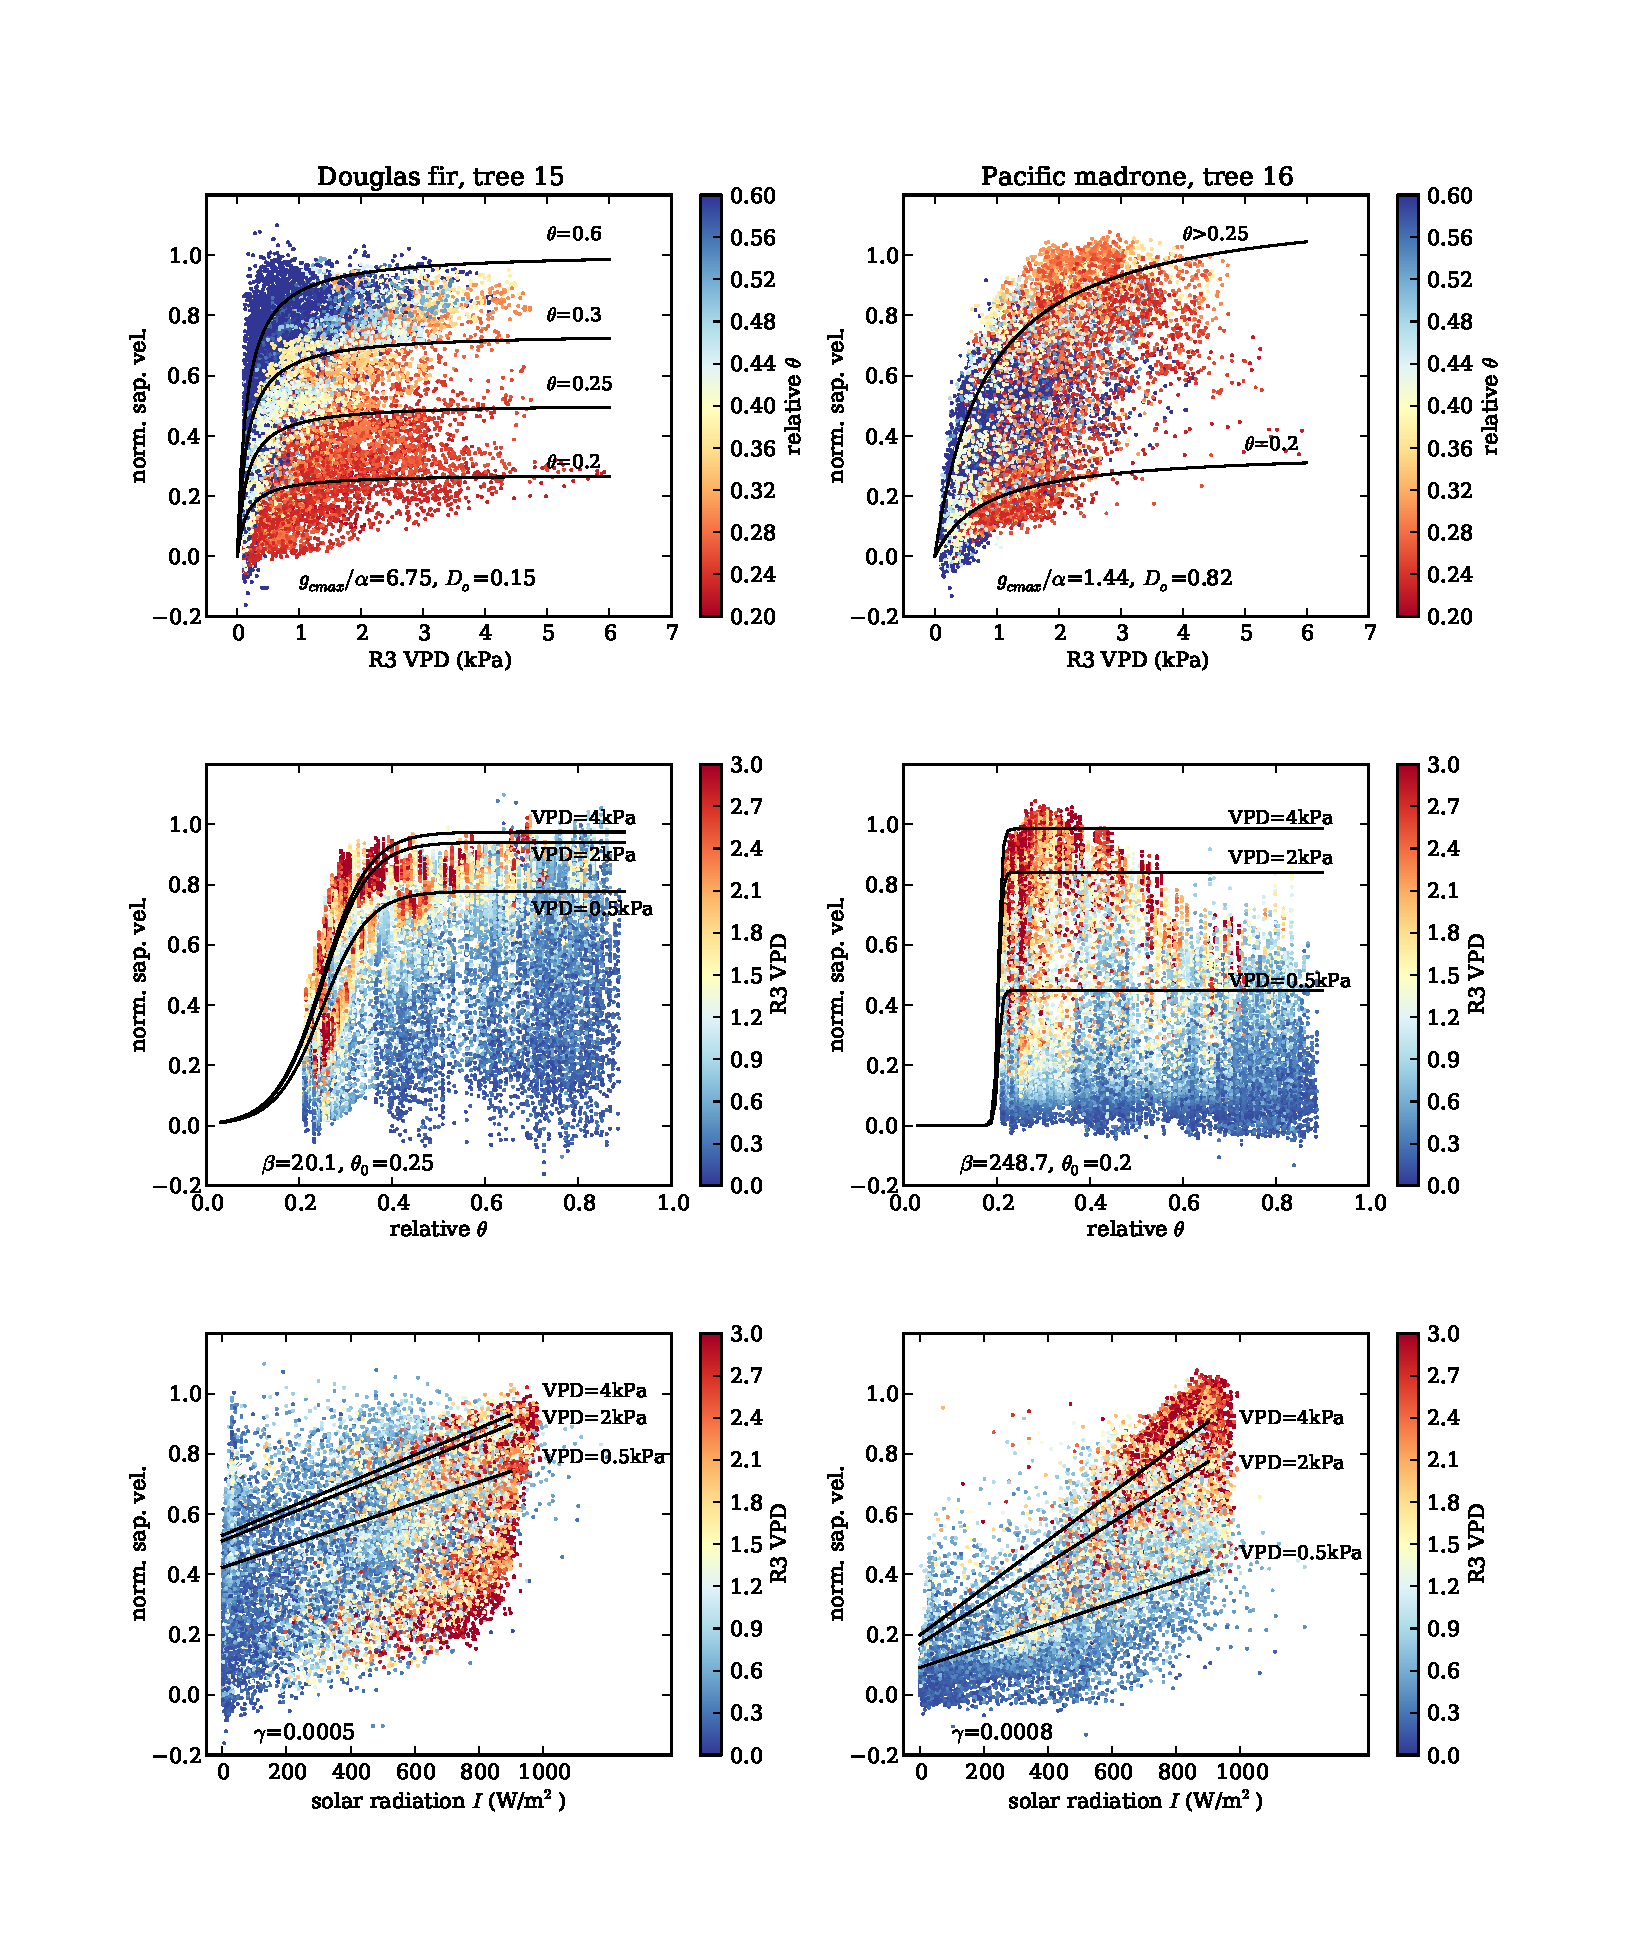
\includegraphics[width=0.9\textwidth]{ch1-sapflow/figures/Figure06.pdf}
\caption{Sap flow response to environmental drivers for example trees.  Left column: tree 15, Douglas fir.  Right column: tree 16, Pacific madrone.  Top row: \textit{VPD} versus normalized instantaneous sap velocity, with symbols colored by site-averaged relative $\theta$.  Lines show the fitted \textit{VPD} function with different cases of soil moisture.  Middle row: site-averaged site-averaged relative $\theta$ versus normalized instantaneous sap velocity, with symbols colored by \textit{VPD}.  Lines show the fitted soil moisture function with different cases of \textit{VPD}.  Bottom row: solar radiation \textit{I} at station AM versus normalized instantaneous sap velocity, with symbols colored by \textit{VPD}.  Lines show the fitted radiation function, with different cases of \textit{VPD}.}
\label{fig:sapflow_scatter}
\end{figure}

Two end-member cases of tree transpiration response to \textit{VPD}, $\theta$, and \textit{I} are shown in Figure \ref{fig:sapflow_scatter}, with Douglas-fir tree 15 in the left column and Pacific madrone tree 16 in the right column.  In the Douglas-fir, sap flow increases sharply with increasing \textit{VPD} at low \textit{VPD} and then plateaus at higher \textit{VPD}; the low value of $D_o$ captures this behavior.  In contrast, the Pacific madrone's sap flow increases more gradually with increasing \textit{VPD}, and the higher value of $D_o$ quantifies this behavior.

The Douglas-fir's higher value of $\theta_o$ shows that this Douglas-fir's sap flow begins to decline at higher values of $\theta$.  The lower value of $\theta_o$ for the Pacific madrone reflects that the Pacific madrone's sap flow does not decline until lower values of $\theta$.  The parameter $\beta$ represents how fast sap flow declines in response to soil moisture limitation, once the decline starts.  Higher $\beta$ (as with the Pacific madrone in Figure \ref{fig:sapflow_scatter}) means a more rapid decline below the threshold, and lower $\beta$ (as with the Douglas-fir in Figure \ref{fig:sapflow_scatter}) means a more gradual decline.

The response of sap velocity to \textit{I} is captured by the slope $\gamma$, which describes how quickly the sap flow increases with increasing \textit{I}.  In Figure \ref{fig:sapflow_scatter}, the Douglas-fir has a low slope, meaning its sap flow remains high at low \textit{I} and increases only slightly with increasing \textit{I}; while the Pacific madrone has a higher positive slope, meaning that it has low sap flow at low \textit{I} and increases more strongly with increasing \textit{I}.

\begin{figure}[here]
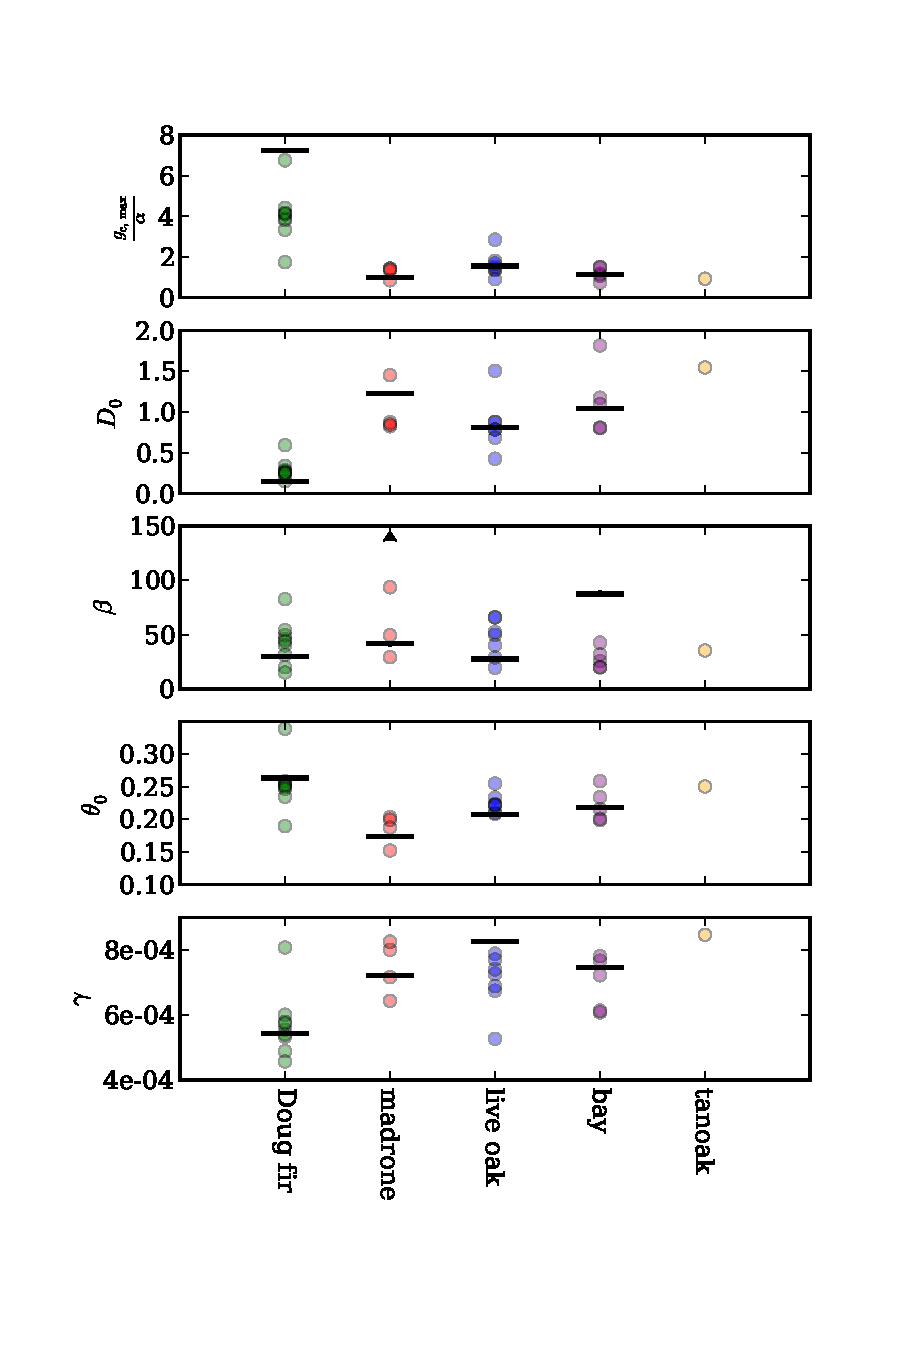
\includegraphics[width=0.65\textwidth]{ch1-sapflow/figures/Figure07.pdf}
\caption{Estimated Jarvis parameters, sorted by species.  Each circle represents the median of the posterior distribution for an individual sensor.  Black horizontal lines show the medians of the posterior distributions for the species-averaged timeseries parameters; vertical black error bars show the 95\% HPD interval (for most species-averaged timeseries parameters, this interval is smaller than the thickness of the horizontal line.)  Row 1: $g_{cmax}/\alpha$ parameter (kPa$^{-1}$), indicating sap velocity at low values of \textit{VPD} and radiation.  Row 2: $D_o$ parameter (kPa), which measures the curvature of the sap velocity increase with increasing \textit{VPD}.  Row 3: $\beta$ parameter (unitless), which measures the rate of sap flow decline around a soil moisture threshold.  The black triangle indicates that one madrone tree has a $\beta$ value higher than 150. Row 4: $\theta_0$ parameter (unitless), which measures the soil moisture value at which sap flow decline is centered.  Row 5: $\gamma$ parameter ((W/m$^2$)$^{-1}$), slope of the sap velocity increase with increasing radiation.}
\label{fig:sapflow_params}
\end{figure}

The Jarvis model parameters for all trees, separated by species, are shown in Figure \ref{fig:sapflow_params} and summarized in Table \ref{tbl:sapflow_mcmc}.  For 25 of the 26 trees, the posterior distributions of all five parameters are sharply peaked and well within the initial uniform prior chosen (example posterior distributions are shown in Figure \ref{fig:sapflow_posterior}).  One Pacific madrone tree (tree 16) has a broader distribution for $\beta$ than other trees (see 95\% HPD interval in Table \ref{tbl:sapflow_mcmc}.)

\begin{table}
  \caption{Median values of estimated Jarvis parameter distributions for each tree, with uncertainties calculated from the 
95\% HPD interval.}
  \label{tbl:sapflow_mcmc}
  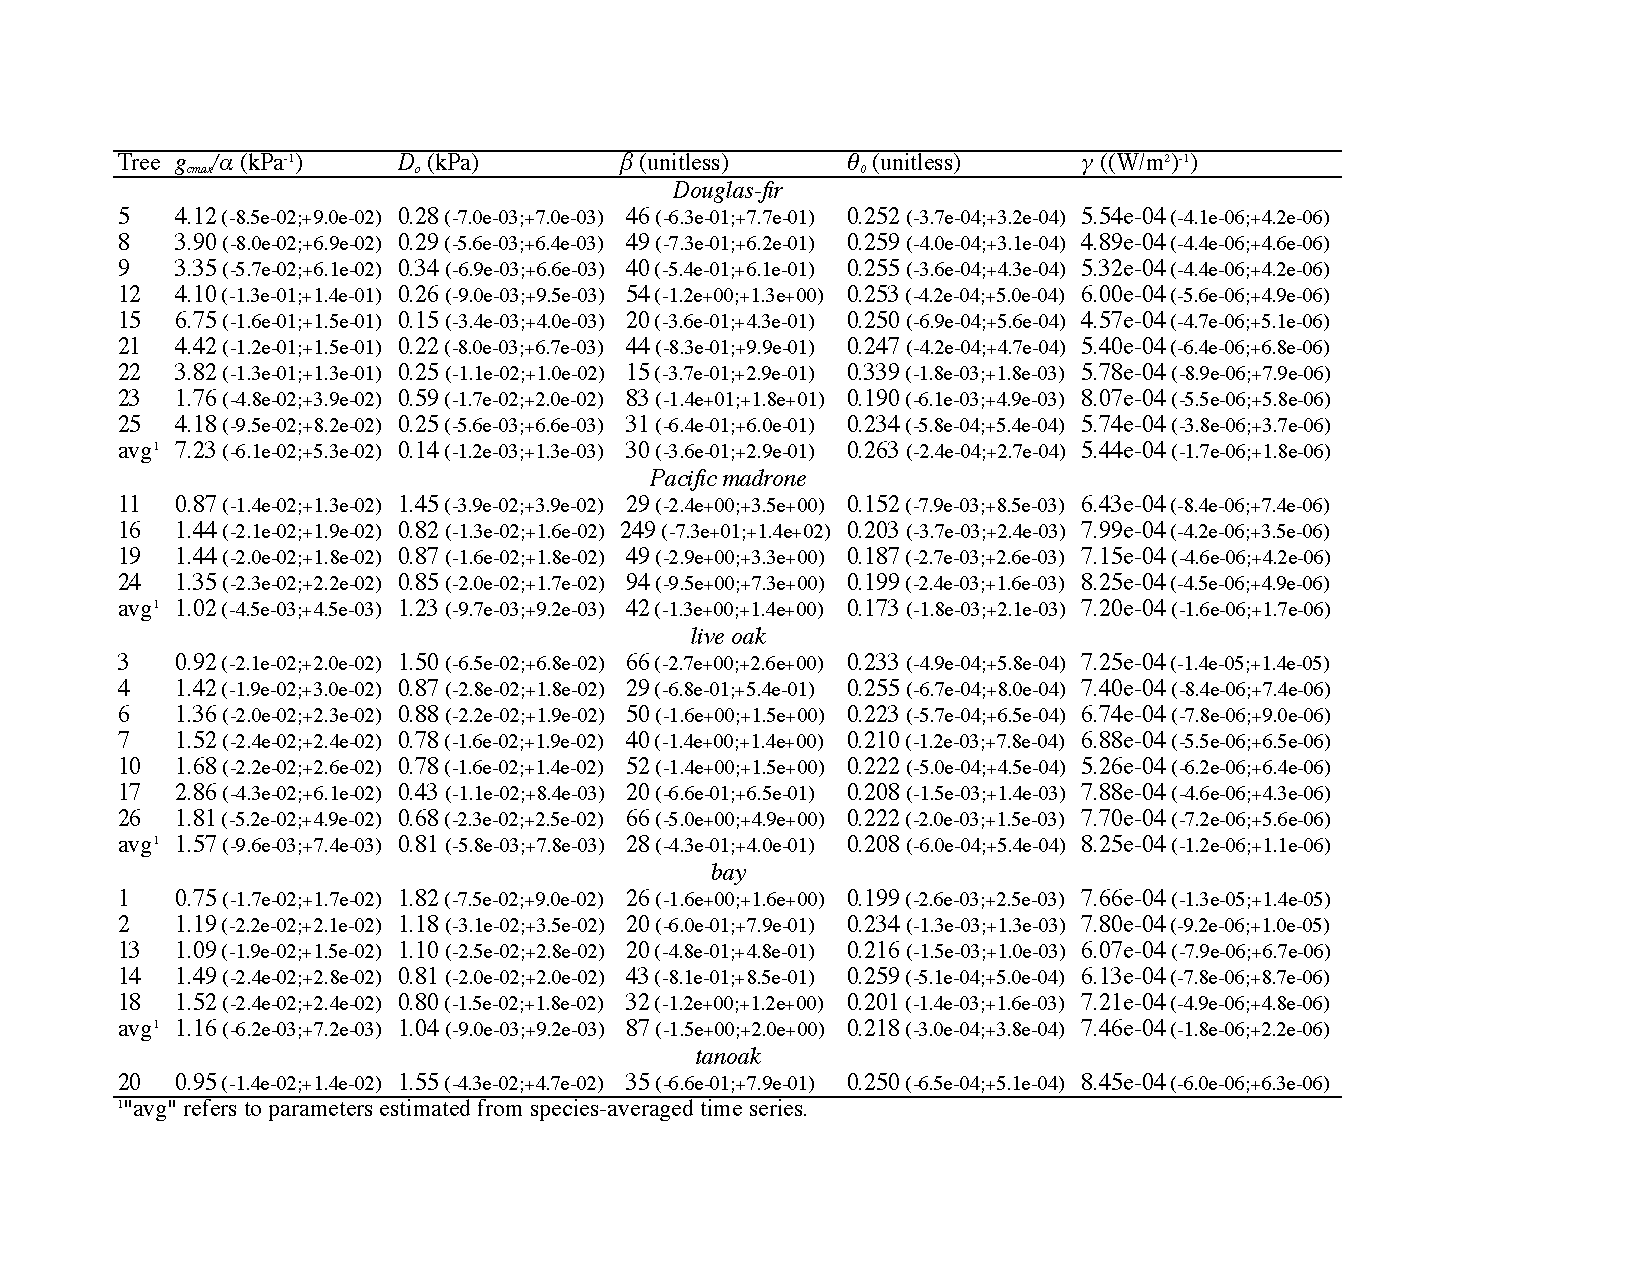
\includegraphics[width=\linewidth]{ch1-sapflow/tables/TableA2}
\end{table}

\begin{figure}[here]
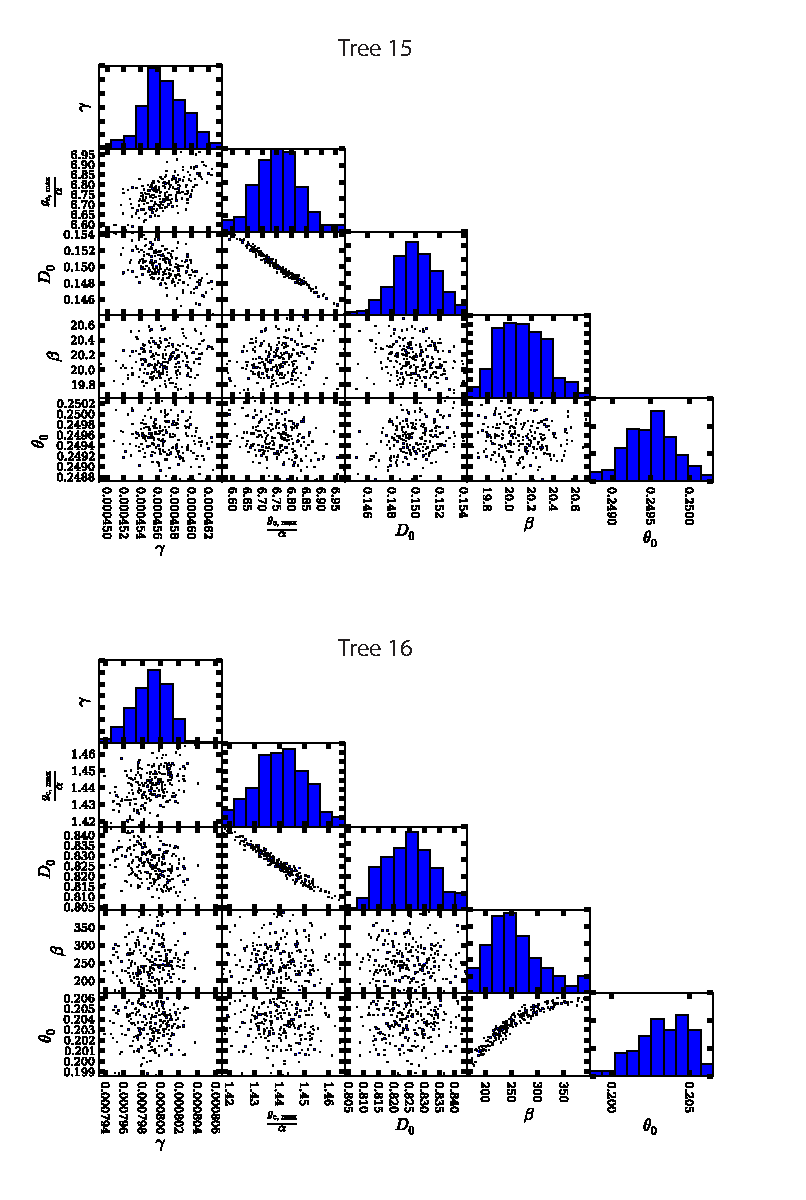
\includegraphics[width=0.75\textwidth]{ch1-sapflow/figures/FigureA1.pdf}
\caption{Panels on the diagonal: posterior distributions of environmental response parameters for the example Douglas-fir sensor (top) and the example Pacific madrone sensor (bottom.)  Panels below the diagonal: covariation of each pair of parameters for each example sensor.}
\label{fig:sapflow_posterior}
\end{figure}

The distributions of the median \textit{VPD} parameters for all sensors and for the species-averaged timeseries parameters ($g_{cmax}/\alpha$ and $D_o$, Figure \ref{fig:sapflow_params}, rows 1 and 2) confirm that sap flow in Douglas-firs across this site increases quickly at low \textit{VPD} and plateaus at high \textit{VPD} (high $g_{cmax}/\alpha$ and low $D_o$).  The broadleaf species, in contrast, respond more gradually with increasing \textit{VPD} (lower $g_{cmax}/\alpha$ and higher $D_o$).

The fitted soil moisture parameter $\theta_o$ (Figure \ref{fig:sapflow_params}, row 4) also shows a species difference.  Douglas-firs have higher $\theta_o$ values; their decline in response to soil moisture limitation is centered on a relative $\theta$ value of 0.263 (from species-averaged timeseries;  $-2.4 \times 10^{-4}$, $+2.7 \times 10^{-4}$ 95\% HPD interval).  Pacific madrones, on the other hand, have lower $\theta_o$ values when fitted to the sigmoid functional form, with declines centered on 0.173 (from species-averaged timeseries; $-1.8 \times 10^{-3}$, $+2.1 \times 10^{-3}$ 95\% HPD interval).

The parameter $\beta$ for individual sensors is more evenly distributed across species, indicating little species difference in the rate of sap flow decline below each individual tree's soil moisture threshold (Figure \ref{fig:sapflow_params}, row 3).  Pacific madrone sensors tend to have higher values of $\beta$, indicating that once their low $\theta_o$ is reached, their transpiration declines sharply; however, $\theta$ values below the Pacific madrone $\theta_o$ values were infrequently observed, so their decline is not well constrained.

The slopes $\gamma$ of the radiation function (Figure \ref{fig:sapflow_params}, row 5) range from $5 \times 10^{-4}$ to $8 \times 10^{-4}$ (W/m$^2$)$^{-1}$.  Douglas-firs tend to have lower slopes, indicating relatively high sap velocity at low \textit{I} and less sensitivity to \textit{I} increase.  In contrast, the broadleaf species (Pacific madrones, live oaks, and bays) have higher slopes, indicating that their sap velocity increases more with increasing \textit{I}.

In general, the parameters do not vary systematically by tree diameter or position on the slope.  There is some increase of $g_{cmax}/\alpha$ and decrease of $D_o$ with increasing tree diameter, but this effect is difficult to disentangle from species differences, because all trees larger than 60 cm in diameter are Douglas-firs, while many of the smaller trees are broadleaf species.  This lack of diameter- and position-dependence is consistent with the PCA results, which suggest that species differences represent the largest contribution to the observed sap flow variability.

The MCMC results show that Douglas-firs and Pacific madrones are at opposite ends of the spectrum of response to \textit{VPD} and $\theta$.  Douglas-firs increase sharply in response to \textit{VPD} and then plateau, while Pacific madrones increase gradually and continually with increasing \textit{VPD}.  Douglas-firs decline significantly at low $\theta$ values, while Pacific madrones show little to no suppression with low $\theta$ values.  Live oaks and bays fall between these end-member responses.

\subsection{Synoptic-scale temporal variability}

\begin{figure}[here]
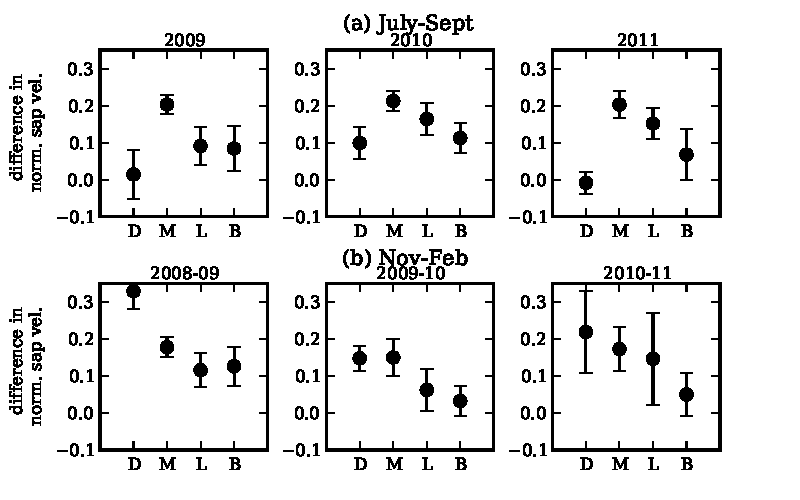
\includegraphics[width=0.9\textwidth]{ch1-sapflow/figures/Figure08.pdf}
\caption{Difference in normalized daily integral sap velocity between high \textit{VPD} days and low \textit{VPD} days, by species (D=Douglas fir, M=Pacific madrone, L=live oak, B=bay).  Circles show mean difference across all trees in the species for that season, and error bars show one standard deviation.  Row (a): July to September, where high \textit{VPD} days are days with maximum \textit{VPD}$>$2 kPa, and low \textit{VPD} days are days with maximum \textit{VPD}$<$2 kPa.  Row (b): November to February, where high \textit{VPD} days are days with maximum \textit{VPD}$>$0.5 kPa, and low \textit{VPD} days are days with maximum \textit{VPD}$<$0.5 kPa.}
\label{fig:sapflow_synoptic}
\end{figure}

The different sensitivity to \textit{VPD} in Douglas-firs and Pacific madrones translates to different transpiration response to synoptic-scale (daily to weekly, weather-scale) variability in atmospheric evaporative demand.  In the summer dry season, \textit{VPD} varies around a high seasonal mean, and the daily maximum value is seldom lower than 1.5 kPa (Figure \ref{fig:sapflow_abundances}(c)).  In this summer range of \textit{VPD} from 1.5 to more than 5 kPa, Douglas-firs have already reached their maximum sap velocity (Figure \ref{fig:sapflow_scatter}(a), for example), but the sap velocity of Pacific madrones, and to a lesser extent live oaks and bays, continues to increase with increasing \textit{VPD}.  Thus, Pacific madrone transpiration is expected to vary significantly in the dry season between high \textit{VPD} and low \textit{VPD} days, while Douglas-fir transpiration should not.  Figure \ref{fig:sapflow_synoptic}(a) shows the summer (July-September) average difference in normalized daily integral sap flow between high \textit{VPD} days (R3 daily max $>$2 kPa) and low \textit{VPD} days (R3 daily max $<$2 kPa) for each species.  Douglas-firs show little to no difference between high \textit{VPD} and low \textit{VPD} days in the summer, while Pacific madrones' sap flow is up to 0.2 normalized units (20\%) higher on high \textit{VPD} days than low \textit{VPD} days.

In the rainy winter, in contrast, \textit{VPD} varies around a much lower seasonal mean, so that the dynamic range of daily maximum \textit{VPD} is 0 to 2 kPa.  In this range, Douglas-firs are highly sensitive to \textit{VPD}, whereas Pacific madrones, live oaks, and bays are less sensitive.  Thus, in the wet winter season, Douglas-firs have greater variability in response to weather-scale \textit{VPD} variation.  Figure \ref{fig:sapflow_synoptic}(b) shows the winter (November-February) average difference in normalized daily integral sap flow between high \textit{VPD} days (R3 daily max $>$0.5 kPa) and low \textit{VPD} days (R3 daily max $<$0.5 kPa).  Douglas-fir sap flow is around 0.2 normalized units (20\%) higher on winter high \textit{VPD} days than low \textit{VPD} days.  Pacific madrones, live oaks, and bays also have higher sap flow on high \textit{VPD} days but by a lesser amount, 0.05-0.15 normalized units (5-15\%).

\subsection{Interannual variability}

\begin{figure}[here]
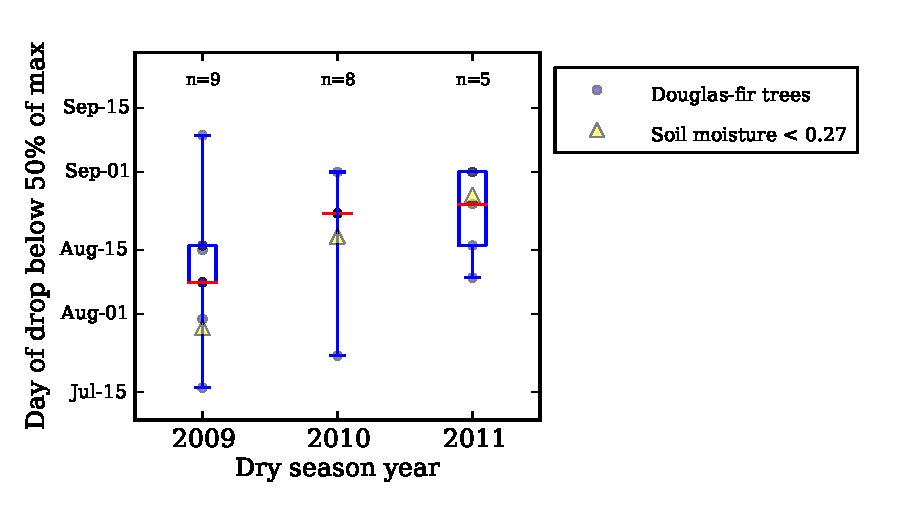
\includegraphics[width=0.9\textwidth]{ch1-sapflow/figures/Figure09.pdf}
\caption{Timing of dry season decline of Douglas-fir trees in each observation year. Each blue dot represents the date of decline below 50\% of a Douglas-fir tree�s maximum daily integral, using only high VPD days (R3 daily max $>$2.5 kPa, linearly interpolating across gaps). The box diagram for each year shows the quartiles of the distribution of all Douglas-fir sensors, with the red line indicating the median. The yellow triangles show the date that site-averaged relative $\theta$ declined below 0.27.}
\label{fig:sapflow_interannual}
\end{figure}

The timing of onset of Douglas-firs' dry season decline varies between years.  Figure \ref{fig:sapflow_interannual} shows the date in each dry season when each Douglas-fir sensor dropped below 50\% of its maximum daily integral, using only high \textit{VPD} days (R3 daily max $>$2.5 kPa, linearly interpolating across gaps), and the box diagrams show the quartiles of the distribution of all Douglas-fir sensors in each year.  The timing of the sap flow decline varies among the three years, occurring approximately two weeks earlier in 2009 than in 2010 or 2011.  The timing of soil moisture depletion also varies among the years, with depletion happening earliest in 2009 and latest in 2011 (yellow triangles in Figure \ref{fig:sapflow_interannual}), largely due to the timing of the last spring storm.  The date of relative soil moisture decline below 0.27 and the median date of Douglas-fir decline below 50\% are close in all three years, although there is notable scatter.

\subsection{Regional transpiration estimates}

\begin{figure}[here]
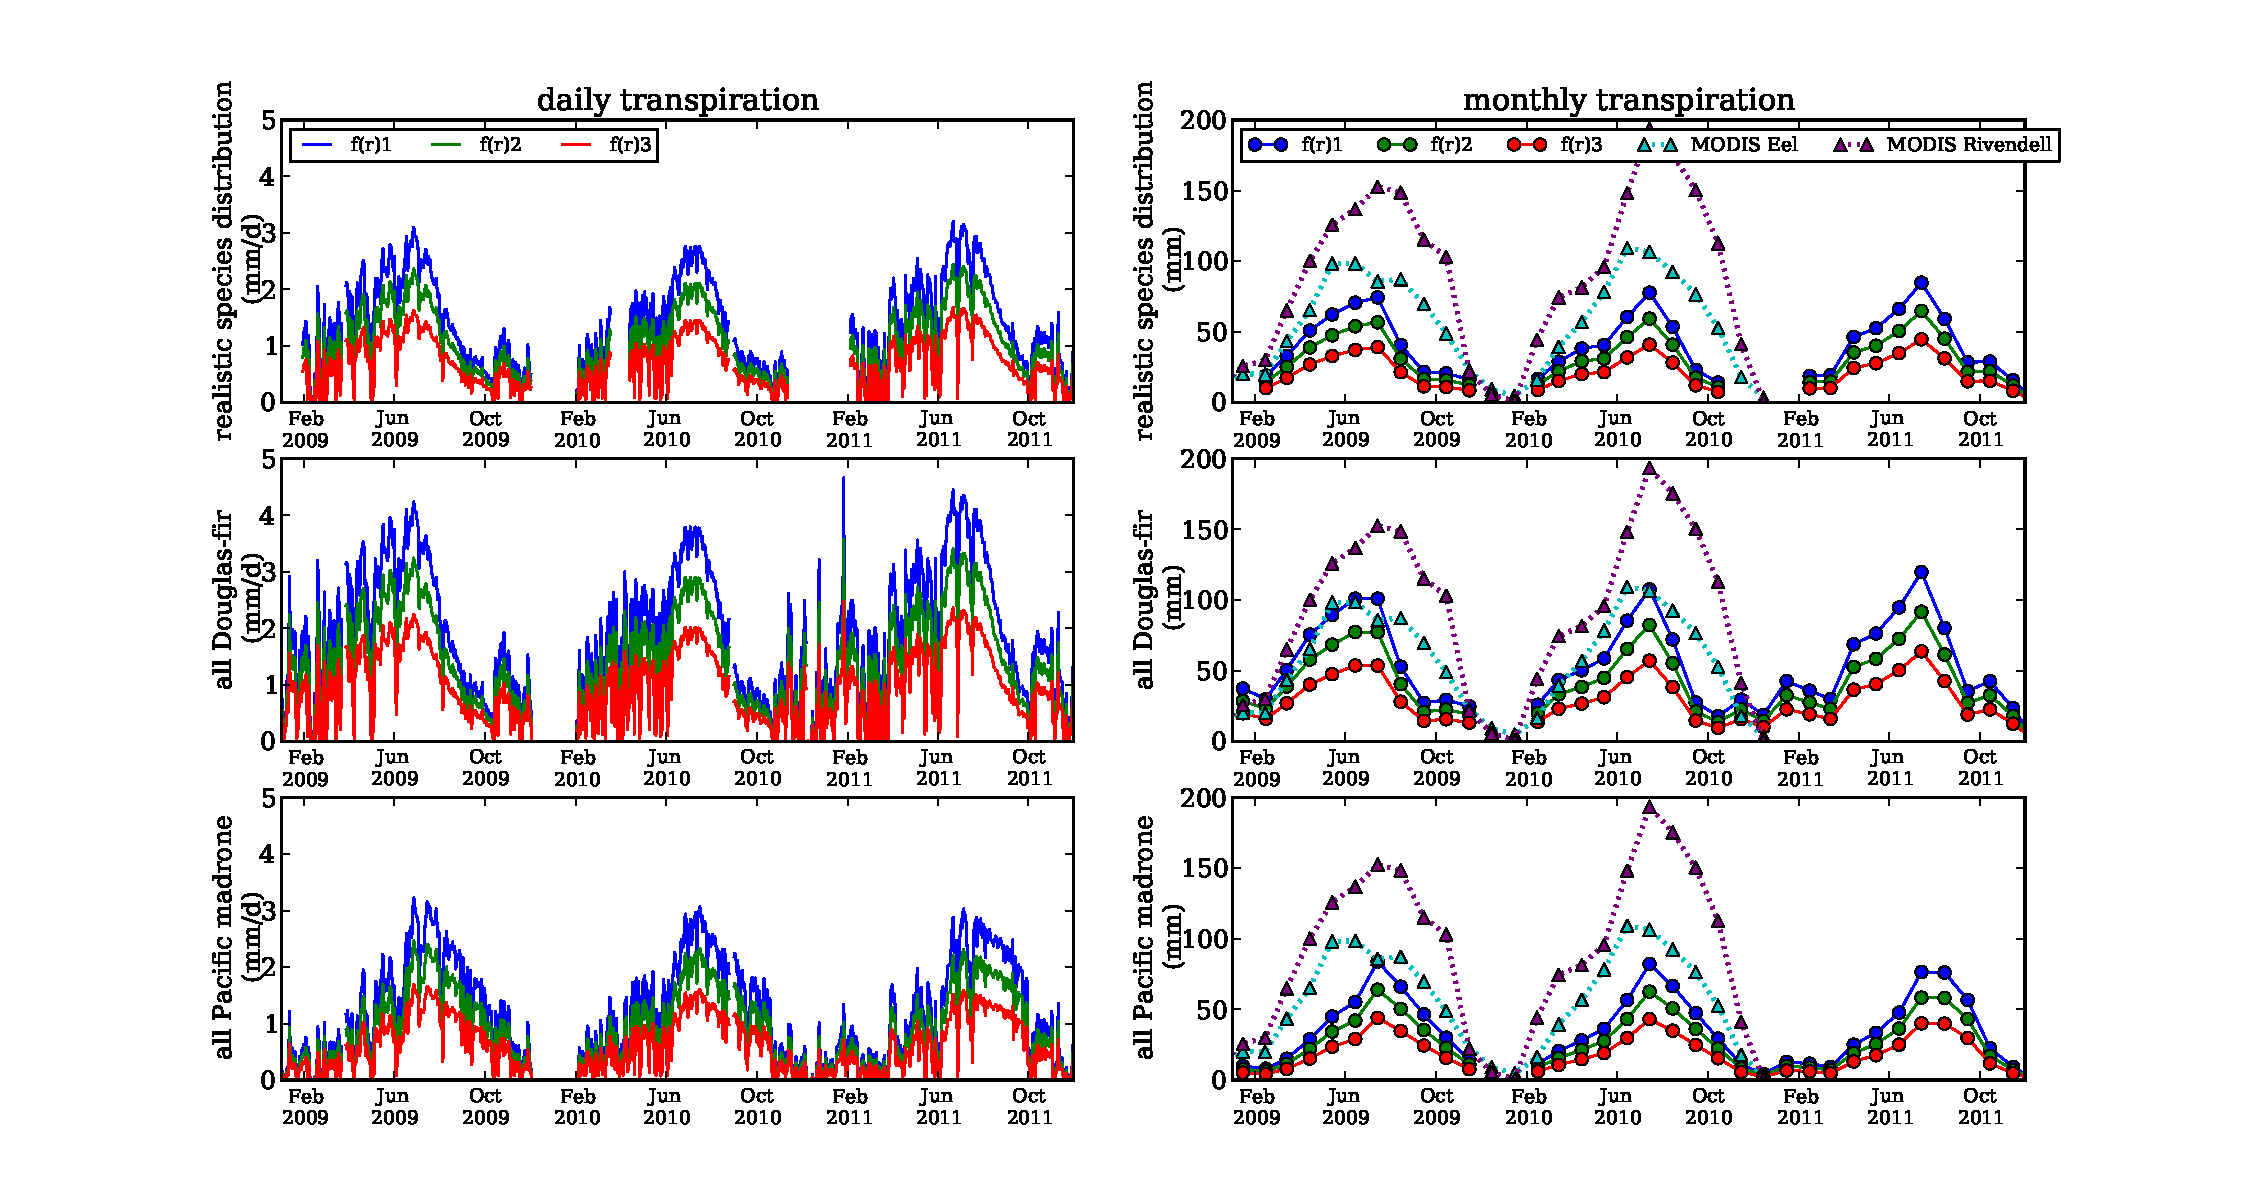
\includegraphics[width=0.9\textwidth]{ch1-sapflow/figures/Figure10.pdf}
\caption{Estimates of regional transpiration.  Left column: daily average transpiration rate estimated for the three plausible radial functions of sap velocity, using a realistic species distribution (top), assuming all trees are Douglas-fir (center), and assuming all trees are Pacific madrone (bottom.)  Right column: monthly integrals of transpiration estimates, again for the three plausible radial velocity profiles, and for the same three cases of species distribution.  Also shown in the right column are remote sensing estimates of monthly ET at two spatial scales: nearest MODIS pixel to the field site (purple), and MODIS estimate averaged over the Eel River watershed (cyan.)}
\label{fig:sapflow_regional}
\end{figure}

Our bottom-up estimates of regional transpiration, estimated with the aid of the FIA data, are shown at daily and monthly timescales in Figure \ref{fig:sapflow_regional} and are compared with a top-down remote sensing estimate of ET derived from MODIS through 2010 in Figure \ref{fig:sapflow_regional}, right column.  Our estimates using a realistic species distribution (row 1) show highest transpiration in June and July and a marked decline in the dry season.  The hypothetical all-Douglas-fir estimate (row 2) is very similar, which is not surprising because a large fraction of trees in the Eel watershed are Douglas-firs, redwoods, or other conifers, and thus the estimate in row 1 is strongly influenced by the Douglas-fir dynamics.  The all-Pacific-madrone hypothetical case (row 3), in contrast, has lower spring (February-May) transpiration and higher dry season (August and September) transpiration than either the realistic species distribution estimate or the all-Douglas-fir estimate.

The three radial sap velocity profiles tested give transpiration estimates that vary by approximately a factor of two.  The upper end of the range is similar in magnitude to the average of MODIS-derived ET for pixels in the Eel watershed (cyan in Figure \ref{fig:sapflow_regional}, right column.)  The sap-flow-based estimates are smaller than the MODIS-derived estimate of ET for the pixel nearest the Rivendell site (purple in Figure \ref{fig:sapflow_regional}, right column) by a factor of 2 to 3.

\begin{figure}[here]
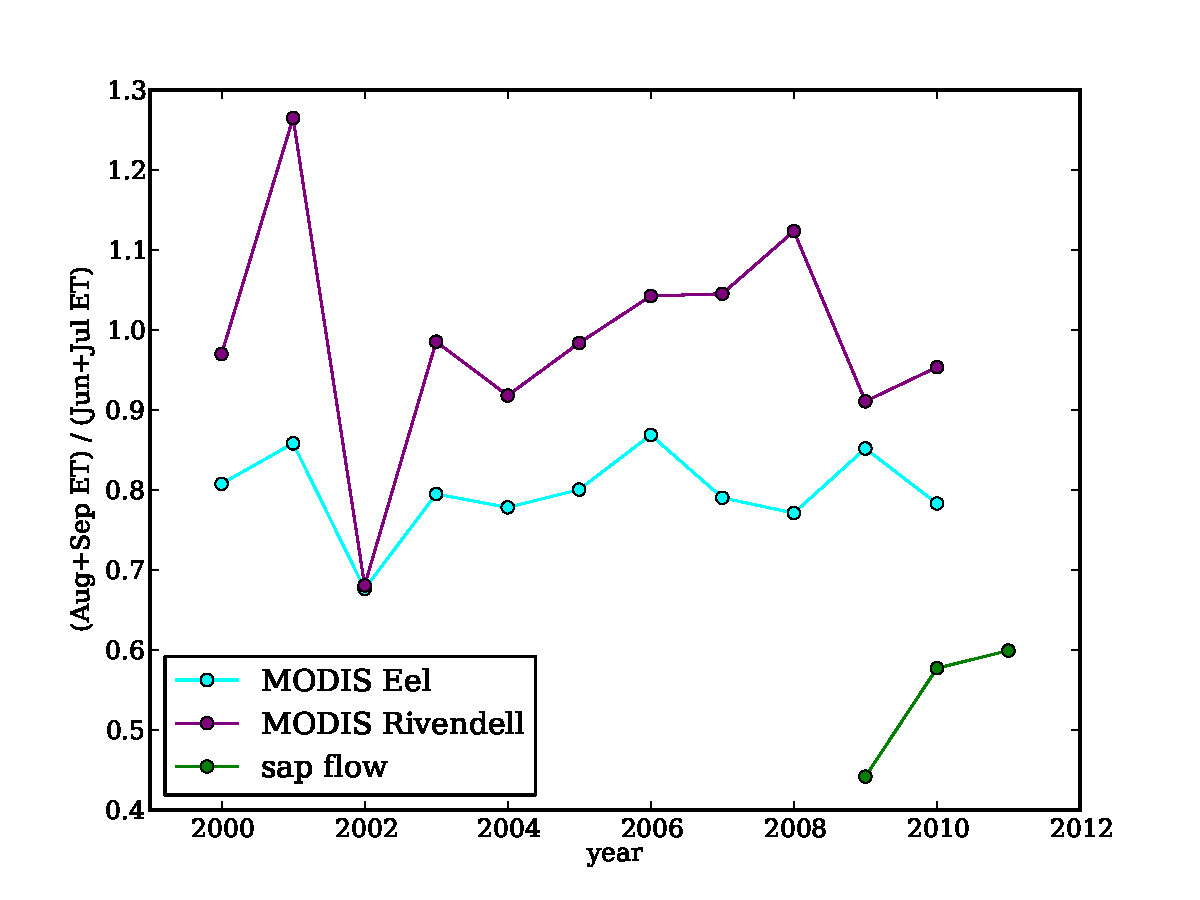
\includegraphics[width=0.9\textwidth]{ch1-sapflow/figures/Figure11.pdf}
\caption{Ratio of dry season to peak season ET (MODIS) or transpiration (sap flow); dry season is defined as August + September, and peak season is defined as June + July.  Two spatial scales are shown for MODIS: the pixel nearest to the Rivendell site (purple) and the average for all pixels in the Eel watershed (cyan.)}
\label{fig:sapflow_ratio}
\end{figure}

With the realistic species distribution, we estimate lower dry season (August-September) transpiration relative to peak (June-July) transpiration than does MODIS.  Figure \ref{fig:sapflow_ratio} shows August plus September transpiration divided by June plus July transpiration for MODIS-derived ET from 2000 to 2010, and for our estimates from 2009 to 2011.  In our estimates, the ratio of dry season transpiration to peak transpiration is the same regardless of radial sap velocity profile (the integral factor in Equation \ref{eqn:transpreg} cancels), so only one sap-flow-based estimate is shown in Figure \ref{fig:sapflow_ratio}.  The MODIS ratio of dry season transpiration to peak transpiration is close to 0.8 for the Eel watershed average and close to 1 for the near-Rivendell pixel for all years and is markedly higher than the sap-flow-based ratio, which is close to 0.5 in all three years.




\section{Discussion}

\subsection{Species difference in response to \textit{VPD} and $\theta$}
Evergreen tree species that coexist on this small hillslope transpire maximally during different seasons.  This difference in transpiration seasonality is due to the species-specific sensitivities of transpiration to atmospheric evaporative demand and subsurface water supply.  Douglas-fir transpiration reaches near-maximum values on clear-sky days in the rainy spring when relative soil moisture exceeds a threshold of $\sim$0.3 even when \textit{VPD} is low (around 1 kPa), and Douglas-fir transpiration declines sharply with the low surface soil moisture conditions of the dry summer.  In contrast, Pacific madrone, live oak, bay, and tanoak transpiration increases continually with increasing \textit{VPD}, reaching maximal transpiration values when atmospheric evaporative demand is highest in the summer dry season; in addition, the low moisture in the upper 50 cm of soil in the summer dry season does not suppress Pacific madrone transpiration and suppresses the other broadleaf species to a lesser degree than it does Douglas-fir.  As a result, Douglas-firs have highest transpiration on clear days in spring, while broadleaf species, and especially Pacific madrones, have highest transpiration on summer days with high atmospheric demand (Figure 4).  The Douglas-fir seasonal pattern is consistent with other studies [\textit{Jassal et al.}, 2009; \textit{Moore et al.}, 2004; \textit{Granier}, 1987]; no studies of Pacific madrone transpiration seasonal patterns were found in the literature.

Sensitivity to \textit{I} also differed between Douglas-firs and the broadleaf species: broadleaf transpiration showed a greater relative increase with increasing \textit{I} than did Douglas-fir transpiration. This species difference might arise in part because, although the parameters are estimated with open-field \textit{I}, trees of different heights on this north-facing slope actually have different access to \textit{I}. Large Douglas-firs (up to 50-60 m tall) generally have greater \textit{I} access than understorey broadleaf trees (20-30 m tall).  Thus, during low \textit{I} times such as mornings or winter days, the large Douglas-firs might have sufficient \textit{I} for photosynthesis and transpiration, while understorey trees might not.

\subsection{Species difference in water access}
It remains uncertain how the broadleaf species and especially Pacific madrones, unlike Douglas-firs, are able to maintain high rates of transpiration during the summer dry period. In order to maintain these high transpiration rates, Pacific madrones must rely either on a more readily available source of water (by placing roots in areas with more moisture, e.g. deeper, or in areas that have higher hydraulic conductivity), or on more-tightly-bound water (by maintaining hydraulic function at lower xylem and leaf water potentials).  There is evidence that Pacific madrones may use both of these mechanisms: at a similar site in southwest Oregon, Douglas-fir roots were confined mainly to the upper 1.5 m of the subsurface, with no roots found below 2.5 m, while Pacific madrones in the same area had notably deeper roots, extending to 2-3.5 m below the surface into rock fissures [\textit{Wang et al.}, 1995; \textit{Zwieniecki and Newton}, 1995;  \textit{Zwieniecki and Newton}, 1996], and Pacific madrones at the Oregon site used water across a greater depth than Douglas-firs [\textit{Zwieniecki and Newton}, 1996].  Moisture in weathered rock can be an important plant water source [\textit{Schwinning}, 2010; \textit{Schwinning}, 2013], and the saprolite zone at our site has significant seasonal variation in water storage and could be an important source for some or all species here [\textit{Salve et al.}, 2012].  Additionally, previous research has shown that Pacific madrones have minimum leaf water potentials of about -3.0 MPa [\textit{Morrow and Mooney}, 1974; \textit{Wang et al.}, 1995], vs. -2.0 MPa in Douglas-firs [\textit{Running}, 1976; \textit{Wang et al.}, 1995]; Pacific madrones' lower minimum leaf water potential suggests that Pacific madrones are less vulnerable to hydraulic failure as soil moisture declines [\textit{Choat et al.}, 2012] and thus might be able to access water bound at low matric potential that is inaccessible to Douglas-fir. Our aboveground sap flow observations cannot distinguish between these two possible mechanisms of water access, but other researchers are using stable isotopes to investigate the water sources for different trees at the site [\textit{Oshun et al.}, 2012], and preliminary results suggest that needleleaf species and broadleaf species use isotopically distinct water sources within the unsaturated zone.  Thus, Douglas-fir (sensitive stomatal control, shallow rooted, and vulnerable to hydraulic failure) and Pacific madrone (less sensitive stomatal control, deeper rooted, and less vulnerable to hydraulic failure) employ contrasting stomatal strategies that are logically connected to hydraulic vulnerability and rooting depth.

We speculate that Pacific madrones may also have higher leaf area during the summer.  Pacific madrone leaves have a lifespan of 14.7 months [\textit{Ackerly}, 2004], meaning that if new leaves emerge at approximately the same time, then for a two- to three-month period each year, the trees might have twice their normal leaf area.  Informal observations at our site indicate that Pacific madrones drop leaves in late summer, so mid-summer may be the high-leaf-area period.  When the leaf area is higher, whole tree transpiration could increase even if transpiration per leaf stayed the same or declined, provided that water stress were not extreme.

Interestingly, Douglas-fir trees at our site do not seem to use groundwater to alleviate water stress during the dry season.  Tree 5, a large Douglas-fir downslope where the water table is $\sim$5 m below ground year-round, declined at a similar rate to upslope Douglas-firs in the dry season (similar soil moisture parameters in Table A2).  Like the instrumented upslope Douglas-firs, tree 5 rebounded strongly with the onset of the rainy season, suggesting water limitation during the dry season until unsaturated zone moisture was replenished by rains.

\subsection{Implications of Douglas-fir water stress}
Douglas-firs' sap flow declined through the dry season in all three years, but the timing of onset of the decline varied between years, corresponding to the timing of moisture decline in the top 50 cm of soil (Figure 9).  The timing of surface soil moisture decline, in turn, seems to depend on the timing of late spring precipitation (Figure 3).  Excess rain during the winter and early spring that exceeds the storage capacity of the soil will run off and have little influence on summer soil moisture availability, but rain in the late spring has the potential to refill a partially empty upper soil reservoir and sustain soil moisture further into the dry season.  Thus, the timing of late spring precipitation is important for sustaining Douglas-fir transpiration through the dry season.  As long as late spring storms meet a certain threshold quantity, their timing may matter more than total wet season precipitation for Douglas-fir function in the dry season.

Douglas-firs may be encroaching on areas formerly dominated by Pacific madrone and other broadleafs in the ACRR, due to a fire-regime shift from controlled burning by indigenous people and early European settlers, to fire suppression in the 20th century [\textit{Johnson}, 1979].  If Douglas-firs become more prevalent, their suppressed transpiration in the dry season could decrease the regional summertime evapotranspiration (Figure 10) and might increase the land surface temperature in the dry season [\textit{Link et al.}, in preparation].  California Coast Range forests with a greater proportion of Douglas fir might also be less resilient to drought, if the Douglas-firs' decline in stomatal conductance reduced whole-tree carbon balance and thus increased sensitivity to subsequent drought events [\textit{McDowell et al.}, 2008].

\subsection{Comparison with previous observations}
Our bottom-up estimate of transpiration agrees generally with the MODIS-derived top-down estimates at the scale of the Eel River watershed (Figure 10).  However, there are important differences in the dry season: we estimate notably lower transpiration in August and September than does the MODIS remote sensing method (Figure 11).  It is unlikely that the difference could be due to soil evaporation unaccounted for in the sap flow method, because surface soils are very dry in the late dry season.  It is possible that other conifer species in the watershed, such as redwood and pine species, have less stomatal closure than Douglas-fir at low soil moisture values, and that our method underestimates transpiration by these other species.  However, \textit{Pinaceae} tend to use water conservatively because they are vulnerable to embolism [\textit{Mart\'inez-Vilalta et al.}, 2004], suggesting that pine species in this region, which make up much of the ``other conifer'' category in Figure 4, would be likely to close their stomata under dry soil conditions like Douglas-firs do.  It is also possible that the FIA inventory underestimates the contribution of broadleaf species like Pacific madrone that transpire heavily in the dry season.  Certainly, broadleaf evergreens dominate transpiration locally on certain hillslopes: the species distribution is highly spatially patterned in the Elder Creek and Eel River watersheds, with broadleaf evergreen trees predominant on south-facing slopes and ridges, and Douglas-firs predominant on north-facing slopes and in valleys [Collin Bode and William Dietrich, personal communication].  As such, south-facing slopes may have higher dry season transpiration than north-facing slopes, creating structured spatial variability in dry season transpiration.  Finally, the MODIS algorithm, which uses remotely sensed LAI and reanalysis meteorology to drive a Penman-Monteith model [\textit{Mu et al.}, 2007], may not accurately account for Douglas-fir stomatal closure when soils are dry, because the MODIS algorithm does not incorporate soil moisture information.  Comparison with ET measured by flux towers suggests that the MODIS-derived annual cycle of ET for Mediterranean sites contains large errors [\textit{Vinukollu et al.}, 2011; one flux tower located in the Sierra Nevada foothills oak savanna and one on the western slope of the Sierra Nevada in a mixed-evergreen coniferous forest].

We note that our estimates also agree with measurements of similar sites made with a variety of methods.  \textit{Salve et al.} [2012] used a water balance to calculate an annual ET at Rivendell (excluding interception losses) of 300-500 mm and summer (June-September) ET  of up to 200 mm.  Our estimate using the realistic species distribution and the first radial velocity profile (blue line in Figure 10, top row) gives annual transpiration of 350-410 mm and June-September transpiration of 150-180 mm.  At a wetter Douglas-fir site in British Columbia using the eddy flux method, \textit{Jassal et al.} [2009] measured similar spring and early summer monthly ET (50-70 mm/month), although late summer ET was greater at the wetter British Columbia site than at Rivendell.  At a Douglas-fir site in western Oregon, \textit{Moore et al.} [2004] used sap flow scaling to estimate Douglas-fir dry season transpiration of 0.5-2.5 mm/day, depending on tree age and time within the dry season; these rates bracket our dry season estimates (top left panel of Figure 10.)  In addition, measurements of oak transpiration at a Mediterranean site agree with the oak sap velocities we measured (\textit{Fisher et al.} [2007] measured peak sap velocities around 6 cm/hr) and the transpiration rates we estimate (\textit{Chen et al.} [2008] report oak tree transpiration of 2-4 mm/day in early- to mid-summer.)

\subsection{Uncertainties and limitations}

\subsubsection{Soil moisture}
In this study, we aggregate measurements of soil moisture from across the hillslope into a single site average.  A spatial pattern in $\theta$ has been observed at this site, with downslope profiles maintaining higher moisture content longer into the dry season [\textit{Salve et al.}, 2012].  However, we choose to compare sap flow to a single, site-averaged value of soil moisture for two reasons: (1) a moisture content--matric potential calibration has not been performed, and the variation of material properties along the slope means that the spatial pattern of moisture content might not directly translate to a spatial pattern of matric potential; (2) the location of roots is uncertain, especially for large trees, which, on this steep slope, have root systems extending great lateral distances and deeply into the hillside, and it is thus difficult to constrain where trees are accessing water (i.e., we cannot weight our average by root density [\textit{Chen et al.}, 2008]).  Thus, we use a single averaged relative $\theta$ as an index of water availability, with the recognition that it imperfectly represents the water available to each individual tree.

The TDR measurements of the top 50 to 70 cm do not measure the water content of the saprolite zone between 1 and 3 m below the surface, which may be an important reservoir of plant-available moisture [\textit{Salve et al.}, 2012].  Unfortunately, the measurements used by \textit{Salve et al.} [2012] to explore the saprolite moisture dynamics are not suited to our analyses in this study because of as-yet-undetermined calibration to moisture content (ERSAS) or low temporal resolution (neutron probe).  We compare tree water use to surface (top 50 to 70 cm) soil moisture because it is readily measured at present; as techniques for quantifying moisture in saprolite and weathered rock advance, tree water use should be compared to those observations as well.

\subsubsection{Sap velocity vs. transpiration}
In treating sap velocity as proportional to transpiration, we assume that (1) the radial profile of sap velocity in the sapwood is constant in time, and (2) the change in storage between the measurement point and the leaves is small.  The first assumption is a reasonable [\textit{Cohen et al.}, 1985; \textit{Nadezhdina et al.}, 2002; \textit{Dragoni et al.}, 2009] but not perfect [\textit{Ford et al.}, 2004] approximation.  The second assumption introduces more error at sub-diurnal timescales, when storage changes and temporal lags in velocity between stem and leaf can be significant [e.g. \textit{Waring and Running}, 1978; \textit{Buckley et al.}, 2011], but in the daily integral, the storage change is less than 5\% in Douglas-fir [\textit{Waring and Running}, 1978]; the daily storage change in other species varies but also tends to be small (negligible in \textit{Larix} and \textit{Picea} [\textit{Schulze et al.}, 1985], and up to 3\% in \textit{Juglans regia} [\textit{Constantz and Murphy}, 1990]).  We neglect this storage contribution to transpiration for simplicity.

Similarly, in converting heat pulse velocity to sap velocity, we treat xylem water content as constant through the year, but xylem water content, especially in Douglas-fir [\textit{Waring and Running}, 1978], may decline during long dry periods.  Our water content measurements were made at the end of the dry season and were thus probably a lower bound.  According to Equation 7 in \textit{Burgess et al.} [2001], an underestimation of water content in the wet season would result in an underestimation of sap velocity during the wet season.

\subsubsection{Regional estimate of transpiration}
We have estimated regional transpiration in order to demonstrate the potential for species differences in response to $VPD$ and $\theta$ to influence transpiration at a regional scale.  The estimate required several simplifying assumptions.  First, species recorded in the FIA dataset were grouped into broad categories of needleleaf and broadleaf, both in order to estimate the maximum potential impact of Pacific-madrone-like behavior in broadleafs and also to accommodate species not measured at the Rivendell site.  This coarse categorization could and should be improved if additional species (especially the common conifers) are instrumented in the future.  Second, the sapwood thickness - DBH relationship is poorly constrained for species other than Douglas-fir (our Pacific madrone relationship was based on only 6 samples, and samples were not collected from other broadleaf species at the site because the hardness of the wood made it prohibitively difficult with the available equipment).  This allometric relationship is expected to vary between sites, species, and trees of different ages [\textit{Eamus et al.}, 2006, p. 42]; as such, this relationship is a significant source of uncertainty in our regional estimate.  Similarly, the radial profile of sap velocity is another significant source of uncertainty, and we attempt to quantify this uncertainty by producing three regional estimates, using three reasonable radial velocity profiles (Figure 10.)  However, any errors due to sapwood thickness and radial velocity profile would not change the seasonality of the transpiration estimates, only the magnitude.

Finally, in using small-scale measurements to estimate the behavior of trees at the regional scale, we neglect heterogeneity among hillslopes.  Our regional estimate does not account for heterogeneous meteorology and water availability, or for variation in response between trees in different locations due to, for instance, genetics, climate during growth, or age distribution.  More sap flow and micrometeorological measurements at different sites within the Eel River watershed, as well remotely sensed observations of vegetation, could integrate such heterogeneity and improve the accuracy of the regional estimate.



\section{Conclusions}
Two evergreen tree species common to forests of the northern Pacific US coast have different seasons of peak transpiration, due to their different responses to atmospheric evaporative demand and soil water limitation.  Douglas-fir transpiration is phase-shifted from the annual cycle of solar radiation toward an earlier season of transpiration, with higher transpiration in the wet spring; this is because Douglas-firs' stomatal conductance is sensitive to water availability and \textit{VPD} and their transpiration thus declines through the dry season.  Pacific madrone transpiration, in contrast, is phase-shifted toward a later season of transpiration, with higher transpiration in the dry summer; this is because broadleaf tree species at this site, especially Pacific madrones, are less sensitive to water stress and maintain greater stomatal conductance at high \textit{VPD}.

The observations of sap flow were combined with a regional forest inventory to construct a bottom-up estimate of regional transpiration.  This estimate highlights the regional-scale impact of needleleaf evergreen stomatal sensitivity to water stress.  The resulting suppression of dry season transpiration could create feedbacks from the forest to atmospheric temperature and humidity, and the nature of these feedbacks would depend on species distribution [\textit{Link et al.}, in preparation].  Better constraints on historical and future changes in Pacific coast forest species composition are needed in order to understand the resulting impacts on the land-atmosphere exchange of water and energy.


\section{Appendix: Markov Chain Monte Carlo}
\label{sec:sapflow_appendix}

The MCMC method we adopt computes the likelihood function, assuming that the sap flow measurement errors are normally distributed, and uses the Metropolis-Hastings algorithm to select new members of the chain from a proposal distribution [e.g., \textit{Sivia} 2006 XXXX]. We used the python PyMC module to execute this analysis [\cite{patil}]. The standard deviation of the measurement error for each sensor was determined from the noise floor of the sensor's power spectrum, using Parseval's theorem; the standard deviation for most sensors was 1-3\%, and the largest standard deviation was 8\%.  The Metropolis-Hastings algorithm guarantees convergence of the Markov chains, but convergence is slow when a high rate of rejection ($>>$50\%) of the proposed values occurs, a common circumstance for problems with a large number of parameters.  We investigated marginalization over errors in the environmental variables (temperature, relative humidity, radiation, and soil moisture) adopting a single test sensor for which this problem was computational tractable.  The most likely parameter values for this test sensor were slightly different from those derived assuming the environmental parameters are perfectly known, but the differences were small compared to the differences between sensors and compared to the range of the parameter space.  The 95\% confidence intervals did not widen noticeably in this test, but the slight differences in median values suggest that the 95\% confidence intervals quoted here underestimate the parameter uncertainties by up to a factor of 3.  However, all parameter distribution widths remained a small fraction of the spread in most likely parameters values derived for each species as a whole.  Thus, while the confidence intervals listed in Table \ref{tbl:sapflow_mcmc} should be viewed as lower limits to the true error for a given tree's parameters, we do not expect unaccounted-for uncertainties in environmental variables to significantly impact our species-wide conclusions.

\begin{table}
  \caption{Limits of uniform prior distributions for Markov chain Monte Carlo estimation of Jarvis model parameters (Equation \ref{eqn:sapflow_jarvis}.)}
  \label{tbl:sapflow_priors}
  \begin{tabular}{l r r}
  \hline
  Parameter & Lower limit & Upper limit \\
  \hline
  $g_{cmax}/\alpha$ (kPa-1) & 0 & 9 \\
  $D_o$ (kPa) & 0 & 2 \\
  $\beta$ (unitless) & 0 & 400 \\
  $\theta_0$ (unitless) & 0 & 0.35 \\
  $\gamma$ ((W/m$^2$)$^{-1}$) & 3x10$^{-4}$ & 9x10$^{-4}$ \\
  \hline
  \end{tabular}
\end{table}

We adopt uniform priors for the proposal distributions of the unknowns, and each chain is initialized with a random value within the prior range.  The adopted priors for the free parameters are given in Table \ref{tbl:sapflow_priors}, and we imposed them after exploration of the full range of parameters.  Following an initial ``burn in" period, we establish convergence and independence following \cite{raftery}.  Figure \ref{fig:sapflow_posterior} shows typical results from this analysis for two example trees.  For both trees, $\frac{g_{\rm c,\,max}}{\alpha}$ and $D_o$ are correlated, consistent with the results of \cite{oren1999survey}; $R^2$ values for $\frac{g_{\rm c,\,max}}{\alpha}$ -- $D_o$ correlation ranged from 0.92 to 0.99 over all trees.  For most madrone trees, $\beta$ and $\theta_0$ covary in a nonlinear way, as shown in Figure \ref{fig:sapflow_posterior} (Tree 16); $\beta$ and $\theta_0$ did not covary in this way for other species.  Other parameters are minimally correlated, and the degree of parameter independence shown in Figure \ref{fig:sapflow_posterior} is typical for all sensors.


%\section*{References}

\bibitem[{\textit{Ackerly}(2004)}]{Ackerly}
Ackerly, D. (2004), Functional strategies of chaparral shrubs in relation to seasonal water deficit and disturbance, 
\textit{Ecol. Monogr.}, \textit{74}(1), 25--44.

\bibitem[{\textit{Aranda}(2000)}]{Aranda}
Aranda, I., L. Gil, and J.~A. Pardos (2000), Water relations and gas exchange in \textit{Fagus sylvatica} L. and \textit{Quercus petraea} (Mattuschka) Liebl. in a mixed stand at their southern limit of distribution in Europe,
\textit{Trees}, \textit{14}, 344--352.

\textit{BALDOCCHI AND XU}

\bibitem[{\textit{Baquedano}(2004)}]{Baquedano}
Baquedano, F.~J., and F.~J. Castillo (2006), Comparative ecophysiological effects of drought on seedlings of the Mediterranean water-saver \textit{Pinus halepensis} and water-spenders \textit{Quercus coccifera} and \textit{Quercus ilex}, 
\textit{Trees}, \textit{20}, 689--700.

\bibitem[{\textit{Black}(1979)}]{Black}
Black, T.~A. (1979), Evapotranspiration from Douglas fir stands exposed to soil water deficits, 
\textit{Water Resour. Res.}, \textit{15}(1), 164--170.

\textbf{BONAN}

\bibitem[{\textit{Bond and Kavanagh}(1999)}]{Bond}
Bond, B.~J., and K.~L. Kavanagh (1999), Stomatal behavior of four woody species in relation to leaf-specific hydraulic conductance and threshold water potential,
\textit{Tree Physiol.}, \textit{19}, 503--510.

\bibitem[{\textit{Brooks}(2006)}]{Brooks}
Brooks, J.~R., F.~C. Meinzer, J.~M. Warren, J.-C. Domec, and R. Coulombe (2006), Hydraulic redistribution in a Douglas-fir forest: lessons from
system manipulations, \textit{Plant, Cell and Environment}, \textit{29}, 138--150.

\bibitem[{\textit{Buckley et al.}(2011)}]{Buckley}
Buckley, T.~N., T.~L. Turnbull, S. Pfautsch, and M.~A. Adams (2011), Nocturnal water loss in mature subalpine \textit{Eucalyptus
delegatensis} tall open forests and adjacent \textit{E. pauciflora}
woodlands, \textit{Ecology and Evolution}, 435--450.

\bibitem[{\textit{Burgess et~al.}(2001)}]{Burgess}
Burgess, S.~S.~O., M.~A. Adams, N.~C. Turner, C.~R. Beverly, C.~K. Ong, A.~A.~H. Khan, and T.~M. Bleby (2001), An improved heat pulse method to measure low and reverse rates of sap flow in woody plants, 
\textit{Tree Physiol.}, \textit{21}, 589--598.

\bibitem[{\textit{\v{C}erm\'{a}k et~al.}(1992)}]{Cermak}
\v{C}erm\'{a}k, J., E. Cienciala, J. Ku\v{c}era, and J.-E. H\"{a}llgren (1992), Radial velocity profiles of water flow in trunks of Norway spruce and oak and the response of spruce to severing, 
\textit{Tree Physiol.}, \textit{10}, 367--380.

\bibitem[{\textit{Chen}(2008)}]{Chen}
Chen, X., Y. Rubin, S. Ma, and D. Baldocchi (2008), Observations and stochastic modeling of soil moisture control on evapotranspiration in a Californian oak savanna,
\textit{Water Resour. Res.}, \textit{44}.

\bibitem[{\textit{Chirino}(2011)}]{Chirino}
Chirino, E., J. Bellot, and J.~R. S\'anchez (2011), Daily sap flow rate as an indicator of drought avoidance mechanisms in five Mediterranean perennial species in semi-arid southeastern Spain,
\textit{Trees}, \textit{25}, 593--606.

\bibitem[{\textit{Choat et~al.}(2012)}]{Choat}
Choat, B., S. Jansen, T.~J. Bodribb, H. Cochard, S. Delzon, R. Bhaskar, S. Bucci, T.~S. Feild, S.~M. Gleason, U.~G. Hacke, A.~L. Jacobsen, F. Lens, H. Maherali, J. Mart\'{i}nez-Vilalta, S. Mayr, M. Mencuccini, P.~J. Mitchell, A. Nardini, J. Pittermann, R.~B. Pratt, J.~S. Sperry, M. Westoby, I.~J. Wright, and A.~E. Zanne (2012), Global convergence in the vulnerability of forests to drought, 
\textit{Nature}, \textit{491}, 752--756.

\bibitem[{\textit{Cohen et~al.}(1985)}]{Cohen}
Cohen, Y., F.~M. Kelliher, and T.~A. Black (1985), Determination of sap flow in Douglas-fir trees using the heat pulse technique, 
\textit{Can. J. For. Res.}, \textit{15}, 422--428.

\textbf{CONSTANTZ AND MURPHY}

\bibitem[{\textit{Dang et~al.}(1997)}]{Dang}
Dang, Q.-L., H.~A. Margolis, M.~R. Coyea, M. Sy, and G.~J. Collatz (1997), Regulation of branch-level gas exchange of boreal trees: roles of shoot water potential and vapor pressure difference, 
\textit{Tree Physiol.}, \textit{17}, 521--535.

\bibitem[{\textit{David}}]{David}
David, T.~S., M.~O. Henriques, C. Kurz-Besson, J. Nunes, F. Valente, M. Vaz, J.~S. Pereira, R. Siegwolf, M.~M. Chaves, L.~C. Gazarini, and J.~S. David (2007), Water-use strategies in two co-occurring Mediterranean evergreen oaks: surviving the summer drought,
\textit{Tree Physiol.}, \textit{27}, 793--803.

\bibitem[{\textit{Dragoni}}]{Dragoni}
Dragoni, D., K.~K. Caylor, H.~P. Schmid (2009), Decoupling structural and environmental determinants of sap velocity, Part II. Observational application,
\textit{Agricultural and Forest Meteorology}, \textit{149}, 570--581.

\bibitem[{\textit{Feddes}}]{Feddes}
Feddes, R., P. Kowalik, and H. Zaradny (1978), \textit{Simulation of Field Water Use and Crop Yield}, John Wiley, New York.

\bibitem[{\textit{Ford et~al.}(2004)}]{Ford}
Ford, C.~R., M.~A. McGuire, R.~J. Mitchell, and R.~O. Teskey (2004), Assessing variation in the radial profile of sap flux density in \textit{Pinus} species and its effect on daily water use,
\textit{Tree Physiol.}, \textit{24}, 241--249.

\bibitem[{\textit{Franks}(2007)}]{Franks}
Franks, P.~J., P.~L. Drake, and R.~H. Froend (2007), Anisohydric but isohydrodynamic: seasonally constant plant water potential gradient explained by a stomatal control mechanism incorporating variable plant hydraulic conductance,
\textit{Plant, Cell and Environment}, \textit{30}, 19--30.

\bibitem[{GLOBE}]{GLOBE}
GLOBE Task Team and others (Hastings, D.~A., P.~K. Dunbar, G.~M. Elphingstone, M. Bootz, H. Murakami, H. Maruyama, H. Masaharu, P. Holland, J. Payne, N.~A. Bryant, T.~L. Logan, J.-P. Muller, G. Schreier, and J.~S. MacDonald), eds. (1999), The Global Land One-kilometer Base Elevation (GLOBE) Digital Elevation Model, Version 1.0. National Oceanic and Atmospheric Administration, National Geophysical Data Center, 325 Broadway, Boulder, Colorado 80303, U.S.A. Digital data base on the World Wide Web (URL: http://www.ngdc.noaa.gov/mgg/topo/globe.html) and CD-ROMs.

\bibitem[{\textit{Granier}(1987)}]{Granier}
Granier, A. (1987), Evaluation of transpiration in a Douglas-fir stand by means of sap flow measurements, 
\textit{Tree Physiol.}, \textit{3}, 309--320.

\bibitem[{\textit{Humphreys et~al.}(2003)}]{Humphreys}
Humphreys, E.~R., T.~A. Black, G.~J. Ethier, G.~B. Drewitt, D.~L. Spittlehouse, E.-M. Jork, Z. Nesic, and N.~J. Livingston (2003), Annual and seasonal variability of sensible and latent heat fluxes above a coastal Douglas-fir forest, British Columbia, Canada, 
\textit{Agricultural and Forest Meteorology}, \textit{115}, 109--125.

\bibitem[{\textit{Jarvis}(1976)}]{Jarvis}
Jarvis, P.~G. (1976), The interpretation of the variations in leaf water potential and stomatal conductance found in canopies in the field, 
\textit{Philos. Trans. R. Soc., B}, \textit{273}, 593--610.

\bibitem[{\textit{Jassal et~al.}(2009)}]{Jassal}
Jassal, R.~S., T.~A. Black, D.~L. Spittlehouse, C. Br\"{u}mmer, and Z. Nesic (2009), Evapotranspiration and water use efficiency in different-aged Pacific Northwest Douglas-fir stands, 
\textit{Agricultural and Forest Meteorology}, \textit{149}, 1168--1178.

\bibitem[{\textit{Johnson}(1979)}]{Johnson}
Johnson, S.~G. (1979), The land-use history of the Coast Range Preserve, Mendocino County, California, 
M.A. thesis, 258 pp., San Francisco State University, San Francisco, May.

\bibitem[{\textit{Jung et~al.}(2010)}]{Jung}
Jung, M., M. Reichstein, P. Ciais, S.~I. Seneviratne, J. Sheffield, M.~L. Goulden, G. Bonan, A. Cescatti, J. Chen, R. de Jeu, A.~J. Dolman, W. Eugster, D. Gerten, D. Gianelle, N. Gobron, J. Heinke, J. Kimball, B.~E. Law, L. Montagnani, Q. Mu, B. Mueller, K. Oleson, D. Papale, A.~D. Richardson, O. Roupsard, S. Running, E. Tomelleri, N. Viovy, U. Weber, C. Williams, E. Wood, S. Zaehle, and K. Zhang (2010), Recent decline in the global land evapotranspiration trend due to limited moisture supply, 
\textit{Nature}, \textit{467}, 951--954.

\bibitem[{\textit{Kumagai}(2012)}]{Kumagai}
Kumagai, T., and A. Porporato (2012), Strategies of a Bornean tropical rainforest water use as a function of rainfall regime: isohydric or anisohydric? 
\textit{Plant, Cell and Environment}, \textit{35}, 61--71.

\bibitem[{\textit{Lindroth and Halldin}(1986)}]{Lindroth}
Lindroth, A., and S. Halldin (1986), Numerical analysis of pine forest evaporation and surface resistance, 
\textit{Agricultural and Forest Meteorology}, \textit{38}, 59--79.

\bibitem[{\textit{Lohammar et~al.}(1980)}]{Lohammar}
Lohammar, T., S. Larsson, S. Linder, and S.~O. Falk (1980), FAST: Simulation models of gaseous exchange in Scots Pine, 
in Structure and Function of Northern Coniferous Forests: An Ecosystem Study, Ecological Bulletins, no. 32, edited by T. Persson,
pp. 505-523, Stockholm.

\bibitem[{\textit{Lorenz}(1956)}]{Lorenz}
Lorenz, E.~N. (1956), Empirical orthogonal functions and statistical weather prediction, 
Scientific Report No. 1, Statistical Forecasting Project, 49 pp., Massachusetts Institute of Technology, Department of Meteorology, Cambridge, MA.

\bibitem[{\textit{Marshall and Waring}(1984)}]{Marshall}
Marshall, J.~D., and R.~H. Waring (1984), Conifers and broadleaf species: stomatal sensitivity differs in western Oregon,
\textit{Can. J. For. Res.}, \textit{14}(6), 905--908.

\bibitem[{\textit{Martinez-Vilalta2}(2003)}]{Martinez-Vilalta2}
Mart\'inez-Vilalta, J., M. Mangir\'on, R. Ogaya, M. Sauret, L. Serrano, J. Pe\~nuelas, and J. Pi\~nol (2003), Sap flow of three co-occurring Mediterranean woody species under varying atmospheric and soil water conditions,
\textit{Tree Physiol.}, \textit{23}, 747--758.

\bibitem[{\textit{Martinez-Vilalta}(2004)}]{Martinez-Vilalta}
Mart\'inez-Vilalta, J., A. Sala, and J. Pi\~nol (2004), The hydraulic architecture of Pinaceae -- a review,
\textit{Plant Ecology}, \textit{171}, 3--13.

\bibitem[{\textit{McDowell et~al.}(2008)}]{McDowell}
McDowell, N., W.~T. Pockman, C.~D. Allen, D.~D. Breshears, N. Cobb, T. Kolb, J. Plaut, J. Sperry, A. West, D.~G. Williams, and E.~A. Yepez (2008), Mechanisms of plant survival and mortality during drought: why do some plants survive while others succumb to drought?, 
\textit{New Phytologist}, \textit{178}, 719--739.

\bibitem[{\textit{Morrow and Mooney}(1974)}]{Morrow}
Morrow, P.~A., and H.~A. Mooney (1974), Drought adaptations in two Californian evergreen sclerophylls, 
\textit{Oecologia}, \textit{15}, 205--222.

\bibitem[{\textit{Mu}(2007)}]{Mu}
Mu, Q., F.~A. Heinsch, M. Zhao, and S.~W. Running (2007), Development of a global evapotranspiration algorithm based on MODIS and global meteorology data, 
\textit{Remote Sensing of Environment}, \textit{111}(4), 519--536.

\bibitem[{\textit{Nadezhdina et~al.}(2002)}]{Nadezhdina}
Nadezhdina, N., J. \v{C}erm\'{a}k, and R. Ceulemans (2002), Radial patterns of sap flow in woody stems of dominant and understory species: scaling errors associated with positioning of sensors, 
\textit{Tree Physiol.}, \textit{22}, 907--918.

\bibitem[{Oleson}]{Oleson}
Oleson, K.~W., D.~M. Lawrence, G.~B. Bonan, M.~G. Flanner, E. Kluzek, P.~J. Lawrence, S. Levis, S.~C. Swenson, P.~E. Thornton, A. Dai, M. Decker, R. Dickinson, J. Feddema, C.~L. Heald, F. Hoffman, J.-F. Lamarque, N. Mahowald, G.-Y. Niu, T. Qian, J. Randerson, S. Running, K. Sakaguchi, A. Slater, R. St\"{o}ckli, A. Wang, Z.-L. Yang, X. Zeng, and X. Zeng (2010), Technical Description of version 4.0 of the Community Land Model (CLM), NCAR Technical Note NCAR/TN-478+ STR, National Center for Atmospheric Research, 257 pp.

\bibitem[{\textit{Oren et~al.}(1999)}]{Oren}
Oren, R., J.~S. Sperry, G.~G. Katul, D.~E. Pataki, B.~E. Ewers, N. Phillips, and K.~V.~R. Sch\"{a}fer (1999), Survey and synthesis of intra- and interspecific variation in stomatal sensitivity to vapour pressure deficit, 
\textit{Plant, Cell and Environment}, \textit{22}, 1515--1526.

\bibitem[{\textit{Oshun}(2012)}]{Oshun}
Oshun, J., D. Rempe, P. Link, K.~A. Simonin, W.~E. Dietrich, T.~E. Dawson, and I. Fung (2012), A look deep inside a hillslope reveals a structured heterogeneity of isotopic reservoirs and distinct water use strategies for adjacent trees, \textit{AGU Fall Meeting Abstracts}, San Francisco, CA.

\bibitem[{\textit{Pataki et~al.}(2000)}]{Pataki}
Pataki, D.~E., R. Oren, and W.~K. Smith (2000), Sap flux of co-occurring species in a western subalpine forest during seasonal soil drought, 
\textit{Ecology}, \textit{81}(9), 2557--2566.

\bibitem[{\textit{Patil et~al.}(2010)}]{Patil}
Patil, A., D. Huard, and C.~J. Fonnesbeck (2010), PyMC: Bayesian stochastic modelling in python,
\textit{J. Stat. Software}, \textit{35}(4), 1--81.

\bibitem[{Raftery}]{Raftery}
Raftery, A.~E., and S.~M. Lewis (1995), The number of iterations, convergence diagnostics, and generic metropolis algorithms, in \textit{Practical Markov Chain Monte Carlo}, W.~R. Gilks, D.~J. Spiegelhalter, and S. Richardson, eds.

\bibitem[{\textit{Rempe et~al.}(2010)}]{Rempe}
Rempe, D., J. Oshun, W. Dietrich, R. Salve, and I. Fung (2010), Controls on the weathering front
depth on hillslopes underlain by mudstones and sandstones, \textit{AGU Fall Meeting Abstracts}, \textit{1},
05.

\bibitem[{\textit{Rodriguez-Iturbe et~al.}(2001)}]{Rodriguez}
Rodriguez-Iturbe, I., A. Porporato, F. Laio, and L. Ridolfi (2001), Intensive or extensive use of soil moisture: plant strategies to cope with stochastic water availability, 
\textit{Geophysical Research Letters}, \textit{28}(23), 4495--4497.

\bibitem[{\textit{Running}(1976)}]{Running}
Running, S.~W. (1976), Environmental control of leaf water conductance in conifers, 
\textit{Can. J. For. Res.}, \textit{6}, 104--112.

\bibitem[{\textit{Salve}(2012)}]{Salve}
Salve, R., D.~M. Rempe, and W.~E. Dietrich (2012), Rain, rock moisture dynamics, and the rapid response of perched groundwater in weathered, fractured argillite underlying a steep hillslope, 
\textit{Water Resour. Res.}, \textit{48}, W11528, doi:10.1029/2012WR012583.

\textbf{SCHULZE 1985}

\bibitem[{\textit{Schwinning}(2010)}]{Schwinning}
Schwinning, S. (2010), The ecohydrology of roots in rocks,
\textit{Ecohydrology}, \textit{3}, 238--245.

\bibitem[{\textit{Schwinning2}(2013)}]{Schwinning2}
Schwinning, S. (2013), Do we need new rhizosphere models for rock-dominated landscapes?,
\textit{Plant Soil}, \textit{362}, 25--31.

\bibitem[{\textit{Sivia}(2006)}]{Sivia}
Sivia, D.~S., and J. Skilling (2006), \textit{Data Analysis: A Bayesian Tutorial}, Oxford University Press, Oxford, UK.

\bibitem[{\textit{Smith}(1966)}]{Smith}
Smith, J.~H.~G., J. Walters, and R.~W. Wellwood (1966), Variation in sapwood thickness of Douglas-fir in relation to tree and section characteristics, \textit{Forest Science}, \textit{1}(12), 97--103.

\bibitem[{\textit{Tan}(1976)}]{Tan}
Tan, C.~S., and T.~A. Black (1976), Factors affecting the canopy resistance of a Douglas-fir forest, 
\textit{Boundary-Layer Meteorology}, \textit{10}, 475--488.

\bibitem[{\textit{Teuling}(2010)}]{Teuling}
Teuling, A.~J., S.~I. Seneviratne, R. St\"{o}ckli, M. Reichstein, E. Moors, P. Ciais, S. Luyssaert, B. van den Hurk, C. Ammann, C. Bernhofer, E. Dellwik, D. Gianelle, B. Gielen, T. Gr\"{u}nwald, K. Klumpp, L. Montagnani, C. Moureaux, M. Sottocornola, and G. Wohlfahrt (2010), Contrasting response of European forest and grassland energy exchange to heatwaves, 
\textit{Nature Geoscience}, \textit{3}, 722--727.

\bibitem[{\textit{Topp}(1980)}]{Topp}
Topp, G.~C., J.~L. Davis, and A.~P. Annan (1980), Electromagnetic determination of soil water content: Measurements in coaxial transmission lines, 
\textit{Water Resour. Res.}, \textit{16}(3), 574--582.

\bibitem[{\textit{USDA}(2005)}]{USDA}
USDA (2005), CALVEG zones and alliances: vegetation descriptions.  \url{http://www.fs.usda.gov/Internet/FSE_DOCUMENTS/fsbdev3_046448.pdf}

\bibitem[{\textit{Vinukollu}}]{Vinukollu}
Vinukollu, R.~K., E.~F. Wood, C.~R. Ferguson, and J.~B. Fisher (2011), Global estimates of evapotranspiration for climate studies using multi-sensor remote sensing data: Evaluation of three process-based approaches,
\textit{Remote Sensing of Environment}, \textit{115}, 801--823.

\bibitem[{\textit{Wang}(1995)}]{Wang}
Wang, Z.~Q., M. Newton, and J.~C. Tappeiner II (1995), Competitive relations between Douglas-fir and Pacific madrone on shallow soils in a Mediterranean climate, 
\textit{Forest Science}, \textit{41}(4), 744--757.

\bibitem[{\textit{Waring}(2011)}]{Waring1}
Waring, R.~H., and J.~J. Landsberg (2011), Generalizing plant--water relations to landscapes, 
\textit{Journal of Plant Ecology}, \textit{4}(1-2), 101--113.

\bibitem[{\textit{Waring}(1978)}]{Waring2}
Waring, R.~H., and S.~W. Running (1978), Sapwood water storage: its contribution to transpiration and effect upon water conductance through the stems of old-growth Douglas-fir, 
\textit{Plant, Cell and Environment}, \textit{1}, 131--140.

\bibitem[{\textit{Warren}(2007)}]{Warren}
Warren, J.~M., F.~C. Meinzer, J.~R. Brooks, J.-C. Domec, and R. Coulombe (2007), Hydraulic redistribution of soil water in two old-growth coniferous forests: quantifying patterns and controls,
\textit{New Phytologist}, \textit{173}, 753--765.

\bibitem[{Williams}]{Williams}
Williams, C., M. Menne, and J. Lawrimore (2012), Modifications to Pairwise Homogeneity Adjustment software to address coding errors and improve run-time efficiency, NCDC Technical Report NCDC No. GHCNM-12-02, National Climatic Data Center, 28 pp.

\bibitem[{\textit{Woudenberg}(2010)}]{Woudenberg}
Woudenberg, S.~W., B.~L. Conkling, B.~M. O'Connell, E.~B. LaPoint, J.~A. Turner, and K.~L. Waddell (2010), The Forest Inventory and Analysis Database: Database description and users manual version 4.0 for Phase 2, Gen. Tech. Rep. RMRS-GTR- 245. Fort Collins, CO: U.S. Department of Agriculture, Forest Service, Rocky Mountain Research Station. 336 p.

\bibitem[{\textit{Zwieniecki}(1995)}]{Zwieniecki}
Zwieniecki, M.~A., and M. Newton (1995), Roots growing in rock fissures: Their morphological adaptation, 
\textit{Plant and Soil}, \textit{172}, 181--187.

\bibitem[{\textit{Zwieniecki}(1996)}]{Zwieniecki2}
Zwieniecki, M.~A., and M. Newton (1996), Seasonal pattern of water depletion from soil--rock profiles in a Mediterranean climate in southwestern Oregon, 
\textit{Can. J. For. Res.}, \textit{26}, 1346--1352.

